\documentclass[11pt,a4paper,twoside,headsepline,numbers=noenddot,toc=bibliography,cleardoublepage=empty,parskip=half,DIV=calc,BCOR=6mm,pagesize=pdftex]{article}
% \documentclass[11pt, twoside, a4paper]{report}


%---------------------------------------------------------
%	Speed up compile time
%---------------------------------------------------------
% uncommenting these lines will disable PDF compression.
% As a result the PDF will be massive (~100MB) but will compile faster.
% Make sure to comment this out when you want to share the PDF.

% \pdfcompresslevel=0
% \pdfobjcompresslevel=0


%---------------------------------------------------------
%	Aditional Packages
%---------------------------------------------------------
\usepackage[german]{babel}
\usepackage{titlepage} % included in the archive and does some styling
\usepackage[absolute]{textpos}
%\usepackage[separate-uncertainty = true]{siunitx} % enable easy SI units with \SI{VALUE}{\meter}
% Note: errors are written like this \SI{10(1)}{\meter} will show up as (10 ± 1) m

\usepackage{subcaption} % To have multiple plots side by side
\usepackage{float}
\usepackage{url} % enable clickable URLs
\usepackage{listings} % to have code blocks in your document
\usepackage{xcolor}
\usepackage{doi}
\usepackage{microtype}
\usepackage{booktabs}
\usepackage{nicefrac} % creates a fraction that is nicer when used in text \nicefrac{1}{2}
\usepackage[acronym]{glossaries} % creates list of acronyms for you and handles everything

% Make acronyms and tell it the file with the acronym definitions
%\makenoidxglossaries

% Maybe you will need some of these, therefore I have not removed them!
% -----------------------
%     Theory part
% -----------------------
\newacronym{snrs}{SNRs}{Supernova Remnants}
\newacronym{ams}{AMS-02}{Alpha Magnetic Spectrometer}
\newacronym{fermilat}{Fermi-LAT}{Fermi Large Area Telescope}
\newacronym{hegra}{HEGRA}{High Energy Gamma Ray Astronomy}
\newacronym{pwn}{PWN}{Pulsar Wind Nebula}
\newacronym{pwne}{PWNe}{Pulsar Wind Nebulae}

\newacronym{hess}{H.E.S.S.}{High Energy Stereoscopic System}
\newacronym{dc}{DC}{Davies-Cotton}
\newacronym{ars}{ARS}{Analogue Ring Samplers}
\newacronym{fov}{FoV}{Field of View}
\newacronym{cta}{CTA}{Cherenkov Telescope Array}
\newacronym{nsb}{NSB}{Night Sky Background}
\newacronym{cog}{CoG}{Centre of Gravity}
\newacronym{adc}{ADC}{Analogue to Digital Converter}

\newacronym{psf}{PSF}{Point Spread Function}
\newacronym{pe}{p.e.}{Photo Electron}
\newacronym{ism}{ISM}{Interstellar Medium}
\newacronym{gzk}{GZK}{Greisen–Zatsepin–Kuzmin}
\newacronym{cmb}{CMB}{Cosmic Microwave Background}
\newacronym{dsa}{DSA}{Diffusive Shock Acceleration}
\newacronym{grbs}{GRBs}{Gamma Ray Bursts}
\newacronym{agn}{AGN}{Active Galactic Nuclei}
\newacronym{sbgs}{SBGs}{Starburst Galaxies}
\newacronym{ic}{IC}{Inverse Compton}
\newacronym{kn}{KN}{Klein-Nishina}
\newacronym{hawc}{HAWC}{High-Altitude Water Cherenkov Observatory}

\newacronym{eas}{EAS}{Extensive Air Showers}
% -----------------------
%     Corsika simtel
% -----------------------
\newacronym{kascade}{KASCADE}{Karlsruhe Shower Core and Array Detector}
\newacronym{egs4}{EGS4}{Electron Gamma Shower system 4}
\newacronym{venus}{VENUS}{Very Energetic NUclear Scattering}
\newacronym{qgsjet}{QGSJET}{Quark Gluon String model with JETs}
\newacronym{dmpjet}{DMPJET}{Dual Parton Model with JETs}
\newacronym{urqmd}{UrQMD}{Ultra relativistic Quantum Molecular Dynamics}


% -----------------------
%     CTA
% -----------------------
\newacronym{lsts}{LSTs}{Large-Sized Telescopes}
\newacronym{msts}{MSTs}{Medium-Sized Telescopes}
\newacronym{ssts}{SSTs}{Small-Sized Telescopes}
\newacronym{vhe}{VHE}{Very High Energy}
\newacronym{checs}{CHEC-S}{Compact High Energy Camera with Silicon \acrshort{pmts}}
\newacronym{asic}{ASIC}{Application Specific Integrated Circuit}
\newacronym{sipm}{SiPM}{Silicon Photomultiplier}
\newacronym{tf}{TF}{Transfer Function}
% Large-Sized telescopes 

\newacronym{tm}{TM}{TARGET-Module}
\newacronym{target}{TARGET}{TeV Array Readout electronics with GSa/s sampling and Event Trigger}
\newacronym{bdt}{BDT}{Boosted Decision Tree}
\newacronym{ct5tea}{CT5TEA}{CTA-TARGET-5TEA version}
\newacronym{ctc}{CTC}{CTA-TARGET-C version}

\newacronym{impact}{ImPACT}{Image Pixel-wise fit for Atmospheric Cherenkov Telescopes}
\newacronym{sc}{SC}{Schwarzschild-Couder}

\newacronym{corsika}{CORSIKA}{Cosmic Ray Simulations for Kascade}
\newacronym{iact}{IACT}{Imaging Air Cherenkov Telescope}
\newacronym{iacts}{IACTs}{Imaging Air Cherenkov Telescopes}
\newacronym{abrir}{ABRIR}{Algorithm for Background Rejection using Image Residuals}
\newacronym{pmt}{PMT}{Photo Multiplier Tube}
\newacronym{pmts}{PMTs}{Photo Multiplier Tubes}
\newacronym{irf}{IRF}{Instrument Response Function}
\newacronym{ecpl}{ECPL}{Power Law with Exponential Cutoff}
\newacronym{logpar}{LogPar}{Logarithmic Parabola}
\newacronym{ts}{TS}{Test Statistic}
\newacronym{mc}{MC}{Monte Carlo}

% -----------------------
%     DACT
% -----------------------
\newacronym{dact}{DesertACT}{Desert Air Cherenkov Telescope}
\newacronym{pde}{PDE}{Photo Detection Efficiency}
\newacronym{rms}{RMS}{Root Mean Square}



% -----------------------
%     HESS
% -----------------------
\newacronym{aod}{AOD}{Atmospheric Optical Depth}
\newacronym{modtran}{MODTRAN}{Moderate resolution atmospheric Transmission software}
\newacronym{aeronet}{AERONET}{Aerosol Robotic Network}
\newacronym{gsf}{GSF}{Global Spline Fit}

% Define some colors for code 
\definecolor{codegreen}{rgb}{0,0.6,0}
\definecolor{codegray}{rgb}{0.5,0.5,0.5}
\definecolor{codepurple}{rgb}{0.58,0,0.82}
\definecolor{backcolour}{rgb}{0.95,0.95,0.92}

% Defines codeblock styles
\lstdefinestyle{mystyle}{
    backgroundcolor=\color{backcolour},   
    commentstyle=\color{codegreen},
    keywordstyle=\color{magenta},
    numberstyle=\tiny\color{codegray},
    stringstyle=\color{codepurple},
    basicstyle=\ttfamily\footnotesize,
    breakatwhitespace=false,         
    breaklines=true,                 
    captionpos=b,                    
    keepspaces=true,                 
    numbers=left,                    
    numbersep=5pt,                  
    showspaces=false,                
    showstringspaces=false,
    showtabs=false,                  
    tabsize=2
}

% Set the maximum depth sections are counted to and shown in the TOC
\setcounter{secnumdepth}{3} % depth of counting
\setcounter{tocdepth}{3} % depth that toc will show 

% new paragraph style with new line
\newcommand{\myparagraph}[1]{\paragraph{#1}\mbox{}\\}


\lstset{style=mystyle}
\renewcommand{\lstlistingname}{Configuration}% Listing -> Configuration

% Toogle between the two to hide or show images
% \usepackage[draft]{graphicx}
\usepackage{graphicx}
\usepackage[utf8]{inputenc} 
\usepackage{upgreek}
\usepackage{titlesec}
\usepackage{physics} % adds easy derivatives etc. 
%\AtBeginDocument{\RenewCommandCopy\qty\SI} % dont know why
\usepackage{amssymb} % more symbols
\usepackage{amsmath} %enables align environment
\usepackage{multirow}


% \usepackage[showframe]{geometry} % Shows margins in pdf if you want to know what's going on
\usepackage{geometry}
\geometry{
    %a4paper,
	left=40mm,
    % right=20mm,
	top=35mm,
    }
\defcaptionname*{german}{\subsectionautorefname}{Abschnitt}
\defcaptionname*{german}{\subsubsectionautorefname}{Abschnitt}

% Declare new commands
\newcommand{\Orafol}{Orafol SC 943}
\newcommand{\gammapy}{\textit{gammapy}}



% \usepackage{eurosym} % offers euro symbol
% % Declare new SI units
% \DeclareSIUnit{\sieuro}{\mbox{\euro}} % Euro
% \DeclareSIUnit{\inch}{\mbox{''}}
% \DeclareSIUnit{\adc}{\mbox{ADC-counts}}
% \DeclareSIUnit{\sample}{\mbox{S}} 
% \DeclareSIUnit{\pe}{\mbox{p.e.}} 
% \DeclareSIUnit{\gauss}{G}



%\usepackage[separate-uncertainty = true]{siunitx}

% Use biblatex
\usepackage[backend=biber,
natbib=true,
maxcitenames = 2,
maxbibnames = 5,
minbibnames = 4, 
sorting=none]{biblatex}

\usepackage{csquotes}

\addbibresource{references.bib}
\setlength\bibitemsep{1.5\itemsep}


% --------------------------------------------------------
% CUSTOM STUFF:
% \usepackage[textsize=tiny]{todonotes}
% \setlength{\marginparwidth}{2cm}
\usepackage{bm}
%---------------------------------------------------------
\usepackage{hyperref} % enable clickable links to sections, figures, etc. 
\PassOptionsToPackage{unicode}{hyperref}
\PassOptionsToPackage{naturalnames}{hyperref}

% Remove the coloured border around autoref links
\hypersetup{%
pdfborder = {0 0 0}
}




\begin{document}	
\pagestyle{empty}

%---------------------------------------------------------
%	Titlepage
%---------------------------------------------------------

% The Titlepage of your Thesis

\begin{center}

    \vspace*{3cm}
 
    \begin{textblock*}{15 cm}(3.5cm, 4cm)
        \Large \bf{Labormessungen der Intensitäteninterferometrie}
    \end{textblock*}

    \begin{textblock*}{15 cm}(3.5cm, 8cm)
        \bf{Bachelorarbeit aus der Physik}
    \end{textblock*}

    \vspace{4cm}
    
    \vspace{1.2cm}
            Vorgelegt von\\
            {\bf Stephen Weybrecht} \\
            \today

    \vspace*{2.5 cm}
    Erlangen Centre for Astroparticle Physics\\
    Friedrich-Alexander-Universität Erlangen-Nürnberg
    \vspace*{1 cm}

    \vspace*{6 cm}
    Betreuer: Prof. Dr. Stefan Funk
    \vspace*{1 cm}

\end{center}

\pagenumbering{gobble}

\clearpage
\mbox{}
\clearpage
\clearpage
\mbox{}
\clearpage
\pagestyle{plain}


%---------------------------------------------------------
%	Table of Contents
%---------------------------------------------------------
% Generate
\newgeometry{
    %a4paper,
	%left=20mm,
    right=40mm,
	top=35mm,
    } 
\tableofcontents
\restoregeometry
\clearpage
\mbox{}
\clearpage
\pagenumbering{arabic}
\setcounter{page}{1}
 
%---------------------------------------------------------
%	Your Work
%---------------------------------------------------------
% This is where your work comes in 

% -------------------------------
% \listoftodos \clearpage
% It is recommended, to import your chapters from a master file for easier management
\section{Einleitung}
\label{sec:Einleitung}
\begin{itemize}
    \item warum II 
    \item warum an HESS?
    \item Beriets durchgeführte Kampagenen, mit welcher beschäftigt sich diese Arbeit (2022)
    \item Es wird kein Einfluss der Kabel auf $\tau_c$ erwartet -> trotzdem wird in HESS beobachtet
    \item Zweck dieser Arbeit -> Unterscuhung im Labor mit mehr Statistik, Entwicklung und Vergleich von Datenanalysemethoden
\end{itemize}
\clearpage
\mbox{}
\clearpage

\section{Theorie}
\label{sec:Theorie}
In diesem Kapitel werden die wichtigsten theoretischen Grundlagen für die folgende Arbeit dargestellt. 
Dafür wird zuerst der Begriff der Kohärenz von Licht eingeführt, welcher anschließend durch die Korrelationsfunktion erster Ordnung mit einer Korrelation der Feldamplituden verknüpft wird. 
Danach wird die Amplitudeninterferometrie am Beispiel des Michelson-Sterninterferometers diskutiert, indem auf die Theorie zur Messung eines Sternendurchmessers eingegangen wird, bis abschließend auf die Nachteile des Amplitudeninterferometers hingewiesen wird. 
In diesem Zuge werden zwei wichtige mathematische Relationen motiviert: Das van Cittert-Zernike-Theorem und das Wiener-Khintchine-Theorem. 
Im letzten Abschnitt wird die Idee hinter der Intensitätsinterferometrie erklärt. 
Dafür werden die Korrelationsfunktion zweiter Ordnung und die Siegert-Relation eingeführt. 
Zudem wird auf die Phänomene Bunching und Antibunching eingegangen und abschließend aufgezeigt, wie eine interferometrische Messung abläuft. 


\subsection{Kohärenz}
\label{ssec:Kohärenz}
Um ein stabiles Interferenzmuster beobachten zu können, ist es wichtig, dass die beiden einfallenden Lichtfelder eine feste Phasenbeziehung zueinander haben. 
Ist dies nicht der Fall, überlagern sich verschiedene Interferenzmaxima und -minima und ergeben ein räumlich und zeitlich unstetiges Muster. 
Um diese Eigenschaft des Lichts besser zu beschreiben, gibt es den Begriff der Kohärenz.
Man unterscheidet zwischen räumlicher und zeitlicher Kohärenz, wobei räumliche die Phasenbeziehung an verschiedenen Orten zur gleichen Zeit und zeitliche Kohärenz die Phasenbeziehung an ein und demselben Ort, aber zu verschiedenen Zeiten quantifiziert. \cite[Kap. 9.2]{hechtOptik2018}
Eine veranschaulichende Skizze ist in \autoref{fig:skizze kohärenz} dargestellt.
\begin{figure}[h]
    \centering
    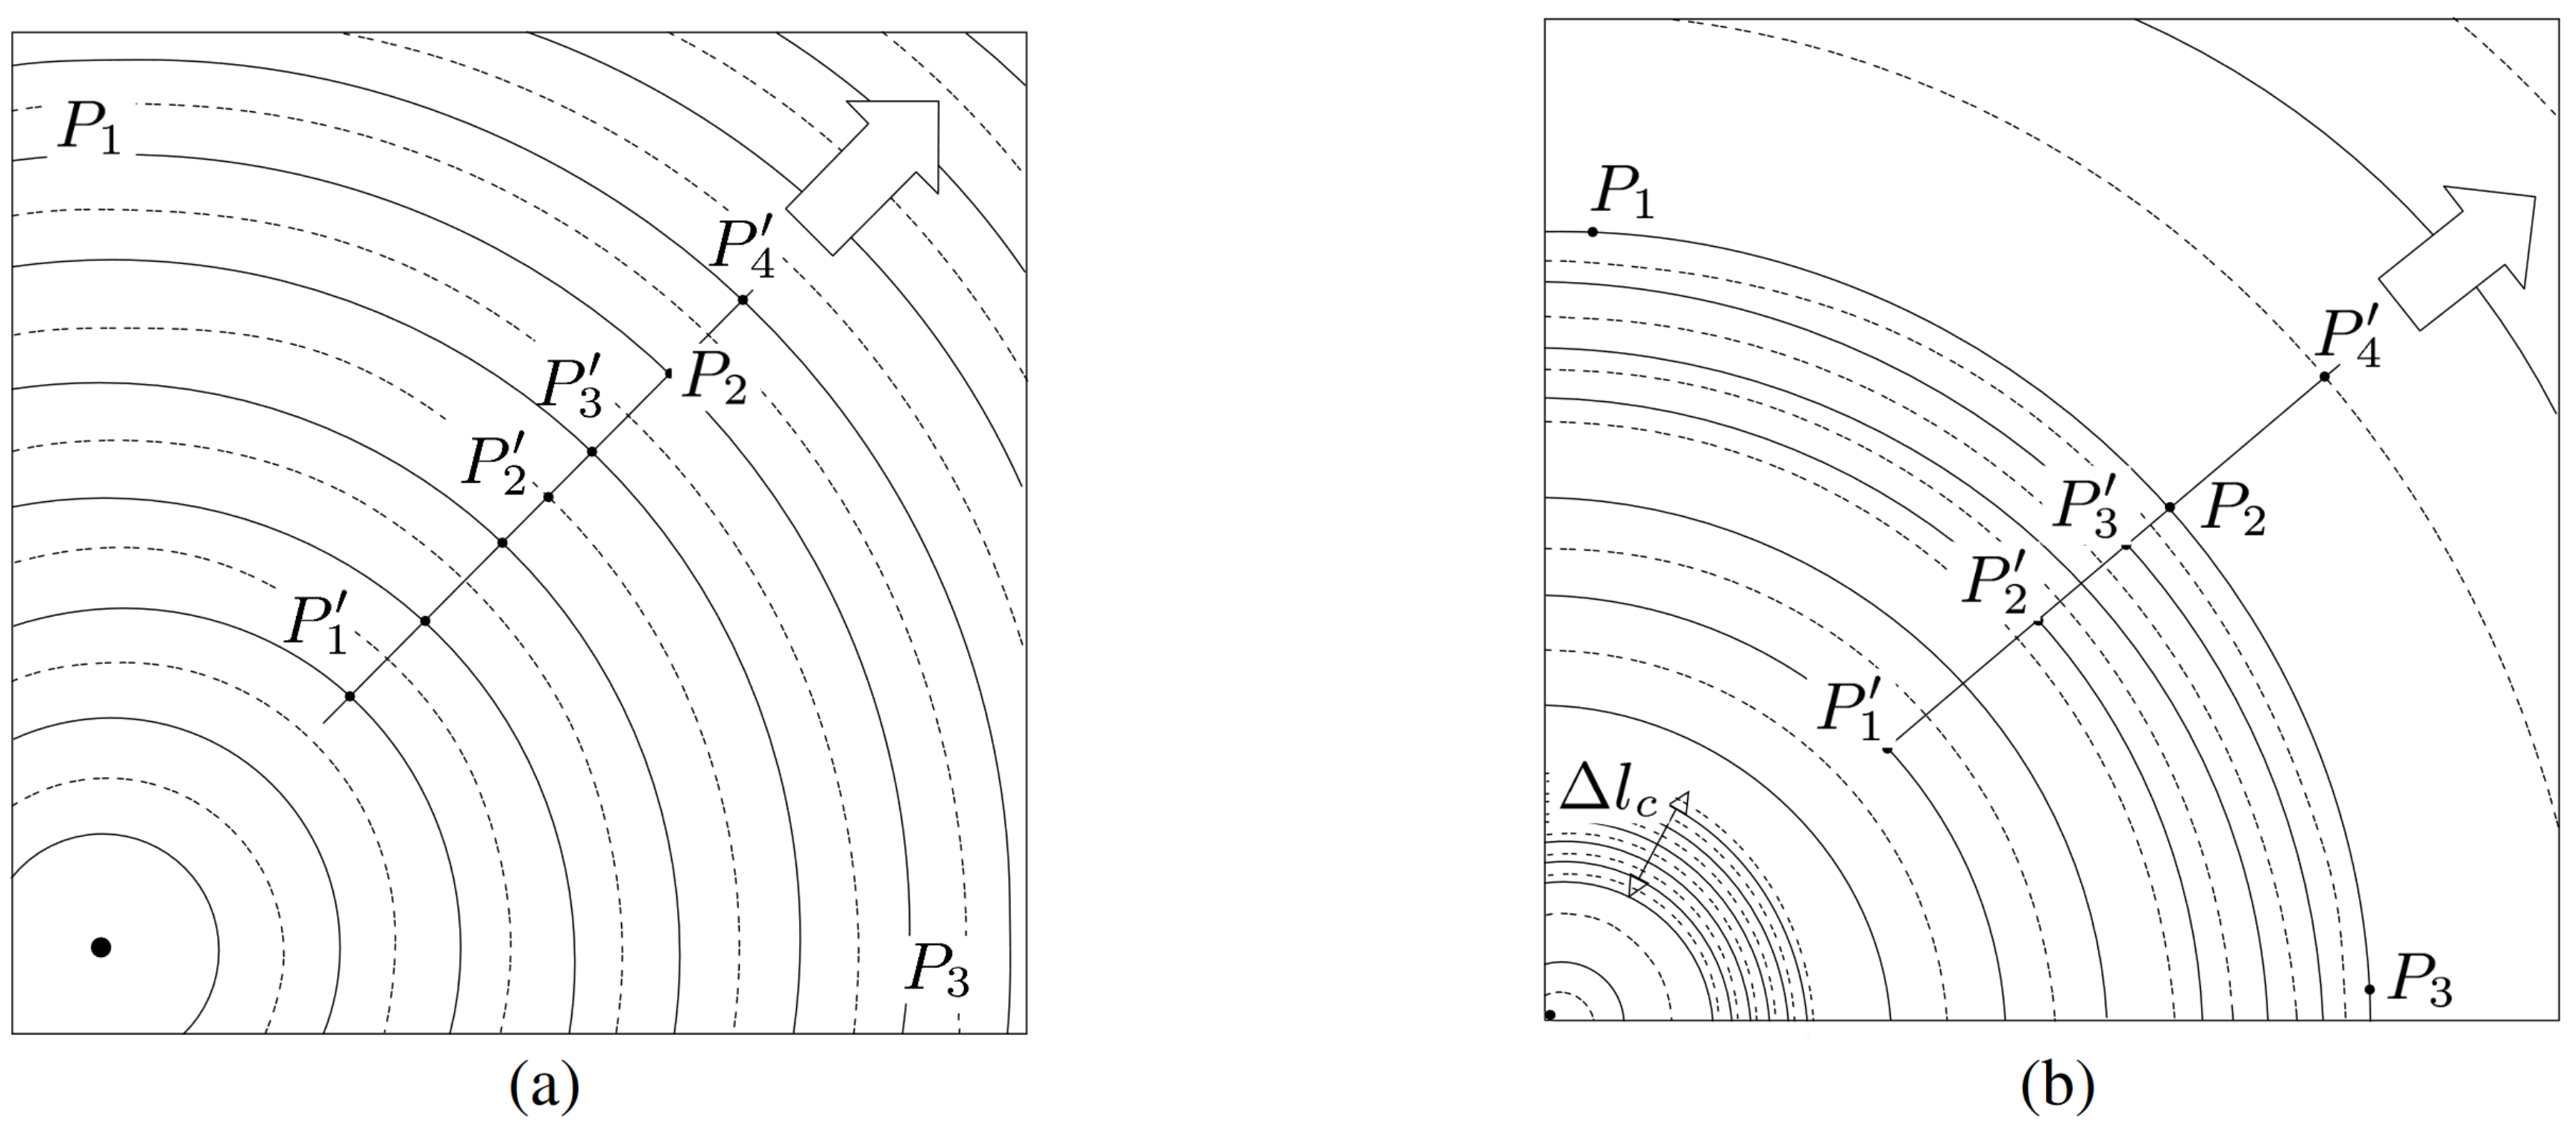
\includegraphics[width=0.8\textwidth]{images/Theorie/Hecht_9.6.png}
    \caption{Dargestellt ist eine Skizze von Wellenfronten zur Veranschaulichung von Kohärenz. In (a) ist die Welle vollständig räumlich und zeitlich kohärent. In (b) ist die Welle nur noch teilweise zeitlich kohärent, aber weiterhin räumlich kohärent. Die Kohärenzlänge $\Delta l_\mathrm{c}$ ist eingezeichnet. Abbildung entnommen aus \cite{hechtOptik2018}.}
    \label{fig:skizze kohärenz}
\end{figure}
\autoref{fig:skizze kohärenz} (a) zeigt eine vollständig kohärente Welle, in welcher Phasenbeziehungen zwischen Punkten in der Ausbreitungsrichtung vollkommen deterministisch sind. 
Die Welle ist monochromatisch und damit zeitlich oder auch longitudinal kohärent. 
Auch in transversaler Richtung (vergleiche Punkte $P_1$-$P_3$) entlang einer Wellenfront ist die Phasenbeziehung für jeden Zeitpukt identisch. 
Die Welle ist räumlich bzw. transversal kohärent. 
Räumliche Kohärenz liegt auch in \autoref{fig:skizze kohärenz} (b) vor. 
Allerdings ist erkennbar, dass die Welle in longitudinaler Richutung nicht für alle Distanzen eine feste Phasenbeziehung aufweist. 
So ist die Frequenz in $P_1'$ beispielsweise niedriger als die in $P_3'$. 
Es existieren aber trotzdem Bereiche, in welchen die Phase sich deterministisch verändert. 
Die kürzeste Länge, für die dies gilt, ist die Kohärenzlänge $\Delta l_\mathrm{c}$, die über die Ausbreitungsgeschwindigkeit $c$ mit der sog. Kohärenzzeit $\Delta l_\mathrm{c} = c\tau_{\mathrm{c}}$ zusammenhängt. 
Die Kohärenzzeit ist damit jene Zeit, für welche die Phase einer Welle vorhersehbar ist. 
Damit haben vollständig zeitlich kohärente Quellen eine unendlich lange Kohärenzzeit, teilweise kohärente Quellen eine endliche Kohärenzzeit, und für inkohärente Quellen gilt $\tau_{\mathrm{c}}\approx 0$. 

Die obige Abbildung motiviert bereits, dass die Kohärenzzeit ein Maß für die spektrale Breite des Lichts $\Delta \omega$ darstellt. 
Es gilt \cite{foxQuantumOpticsIntroduction2006}:
\begin{equation}
    \tau_{\mathrm{c}}  \approx \frac{1}{\Delta \omega}
    \label{eq:tau(delta nu)}
\end{equation}
Da Kohärenz eine Korrelation in den Feldamplituden beschreibt, lässt sich diese Eigenschaft des Lichtes mathematisch mit der sog. Korrelationsfunktion erster Ordnung beschreiben. 
Diese lautet \cite{foellmiIntensityInterferometrySecondorder2009}:
\begin{equation}
    g^{(1)}(\mathbf{r_1}, t_1, \mathbf{r_2}, t_2) = \frac{\left<E^*(\mathbf{r_1}, t_1)E(\mathbf{r_2}, t_2)\right>}{\left[\left<E^*(\mathbf{r_1}, t_1)^2\right> \left<E(\mathbf{r_2}, t_2)^2\right>\right]^{1/2}}
    \label{eq:g1(r1,t1,r2,t2)}
\end{equation}
Hierbei bezeichnet $E(\mathbf{r_i},t_i)$ die komplexe Feldamplitude am Beobachtungsort $\mathbf{r_i}$ und zur Zeit $t_i$ und $\left<\dots\right>$ den Zeitmittelwert über viele Schwingungsperioden. 

Unter der (für weit entfernte, kleine Quellen gerechtfertigten) Annahme, dass die Zeitmittelwerte der Intensitäten an den beiden Orten $\mathbf{r_1}$ und $\mathbf{r_2}$ identisch sind und dass die Intensität zeitlich konstant ist ($\left<I(t_1)\right>=\left<I(t_2)\right>=:I$) lässt sich die Funktion weiter umschreiben. 
Zudem sind häufig nur Differenzen in der Zeit und im Ort relevant, anstatt absolute Orte und Zeiten zu betrachten, was folgende Variablensubstitution nahelegt: $\tau = t_2 -t_1$ und $\bm{\rho} = \mathbf{r_2} - \mathbf{r_1}$. 
Damit folgt:
\begin{equation}
    g^{(1)}(\mathbf{r}, \bm{\rho}, t, \tau) = \frac{\left<E^*(\mathbf{r}, t)E(\mathbf{r}+\bm{\rho}, t+\tau)\right>}{I}
    \label{eq:g1(r1,r2,tau)}
\end{equation}
Häufig wird zudem nur die Korrelation zweier Punkte am selben Ort, d. h. $\bm{\rho}=0$ oder zur selben Zeit, d. h. $\tau=0$, betrachtet. 
Ist dies der Fall, vereinfacht sich \autoref{eq:g1(r1,r2,tau)} zur zeitlichen bzw. räumlichen Korrelationsfunktionen $g^{(1)}(\tau)$ bzw. $g^{(1)}(\bm{\rho})$.


\subsection{Michelson-Sterninterferometer}
\label{ssec:Michelson-Sterninterferometer}
Eine Methode, die räumliche Korrelationsfunktion erster Ordnung zu messen, ist das Michelson-Sterninterferometer, welches schematisch in \autoref{fig:Michelson-Sterninterferometer} dargestellt ist. 
\begin{figure}[h]
    \centering
    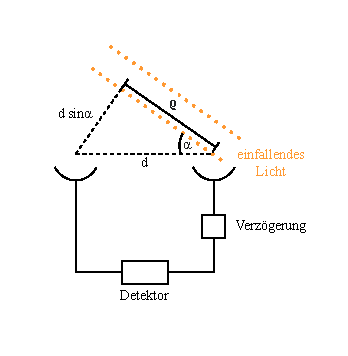
\includegraphics[width=0.65\textwidth]{images/Theorie/Michelson_Interferometer.pdf}
    \caption{Abgebildet ist eine Skizze des Michelson-Sterninterferometers zur Bestimmung von Sternendurchmessern. Zwei durch die Distanz $d$ getrennte Spiegel lenken das Sternenlicht zusammen und es kommt zur Interferenz, die mit einem Detektor beobachtbar ist. Dafür wird der geometrische Streckenunterschied $d\sin\alpha$ durch Verzögerungen kompensiert, um dieselbe Wellenfront zu vergleichen. Abbildung inspiriert von \cite[Abb. 1]{foellmiIntensityInterferometrySecondorder2009}.}
    \label{fig:Michelson-Sterninterferometer}
\end{figure}
Der historische Grund für die Entwicklung von Interferometern zur Beobachtung von Sternen liegt im Ziel, immer bessere Winkelauflösungen erreichen zu wollen. 
Während für die Winkelauflösung gewöhnlicher Teleskope $\theta \propto \frac{\lambda}{D}$ gilt, gilt für Interferometer $\theta \propto \frac{\lambda}{d}$. 
\todo{citation}
Hierbei ist $\lambda$ die Wellenlänge, $D$ der Durchmesser der Teleskopöffnung (je nach Bauart der Hauptspiegel oder die Linse) und $d$ der Abstand zwischen Teleskopen, die ein Interferometer bilden. 
Da es technisch schwierig ist, beliebig große Spiegel- bzw. Linsendurchmesser anzufertigen, sind optische Teleskope auf eine vergleichsweise geringe Auflösung im Bereich von einigen Bogensekunden limitiert. 
Bogensekunden und Bogenminuten (arcsec bzw. arcmin) sind eine typische astronomische Einheit für scheinbare Durchmesser von Objekten in einer gegebenen Entfernung. 
Eine Bogensekunde entspricht dabei dem Sechzigsten Teil einer Bogenminute und eine Bogenminute dem Sechzigsten Teil eines Grades. 
So erreicht z. B. das \emph{Gran Telescopio Canarias} (GTC) eine Auflösung von etwa 12\,marcsec bei $\lambda=500\,\mathrm{nm}$ und $D=10{,}4\,\mathrm{m}$ \cite{GranTelescopioCANARIAS}. 
Obwohl es Bestrebungen gibt, immer größere Einzelspiegelteleskope zu bauen, besteht eine weitere, technisch einfachere Herangehensweise darin, das Licht vieler kleiner Teleskope zu kombinieren. 
Dies ist die Grundidee des Michelson-Sterninterferometers, welches aus zwei Teleskopen besteht, die durch eine Distanz $d$ voneinander getrennt sind. 
Diese bündeln das Licht, welches anschließend zusammengeführt und zur Interferenz gebracht wird. 
Durch dieses Vorgehen lassen sich deutlich bessere Winkelauflösungen bewerkstelligen. 
So erreichte z. B. das Ende der 1980er gebaute \emph{Sydney University Stellar Interferometer} (SUSI) Auflösungen von $70\,\mathrm{\mu arcsec}$ bei $\lambda=450\,\mathrm{nm}$ und $d=640\,\mathrm{m}$ \cite{davisSydneyUniversityStellar1999}. 
Ein Nachteil des Interferometers ist allerdings eine niedrigere Sensitivität im Vergleich zu gewöhlichen Teleskopen. 
Da die Lichtsammelfläche zweier kleiner Teleskope für gewöhnlich kleiner ist als die eines großen Einzelspiegels, wird weniger Licht gesammelt, was interferometrische Verfahren auf vergleichsweise helle Sterne limitiert \cite[Kap. 6.1]{foxQuantumOpticsIntroduction2006}. 
Weiterhin wird statt eines zweidimensionalen Bildes lediglich eine eindimensionale Größe, nämlich der Winkeldurchmesser des Sternes, bestimmt. 
Durch den Zusammenschluss vieler Teleskope kann allerdings trotzdem auf die zweidimensionale Helligkeitsverteilung rückgeschlossen werden. 
Weiterführendes findet man unter dem Stichpunkt \glqq Aperture Synthesis\grqq\;z. B. in \cite[Kap. 10]{burkeIntroductionRadioAstronomy2019}. \\

Beobachtungsziel des Interferometers ist ein Stern, also eine ausgedehnte, thermische Lichtquelle. 
Thermisches Licht ist zwar grundsätzlich nicht kohärent, aber ein Gedankenexperiment zeigt auf, dass durch das Samplen des Lichts an zwei weit vom Stern entfernten Orten trotzdem teilweise Kohärenz vorliegen kann. 
Man kann sich eine ausgedehnte Lichtquelle als die Superposition vieler infinitesimal kleiner Quellen vorstellen. 
Jede dieser Punktquellen hat für sich genommen keine Winkelausdehnung und bildet damit im Fernfeld eine vollständig räumlich kohärente ebene Welle \cite[Kap. 6.1]{foxQuantumOpticsIntroduction2006}. 
Die Überlagerung der Punktquellen bedeutet nun im Fernfeld eine Überlagerung vieler für sich genommen räumlich kohärenten, aber untereinander inkohärenten ebenen Wellen. 
Da in jedem Teleskop des Interferometers eine Vielzahl dieser ebenen Wellen detektiert wird, verbleibt eine gewisse Ähnlichkeit zwischen den detektierten Feldern -- die beiden Felder sind teilweise korreliert. 
Dies ist in \autoref{fig:räumliche kohärenz einer ausgedehnten quelle} dargestellt. 
\begin{figure}[h]
    \centering
    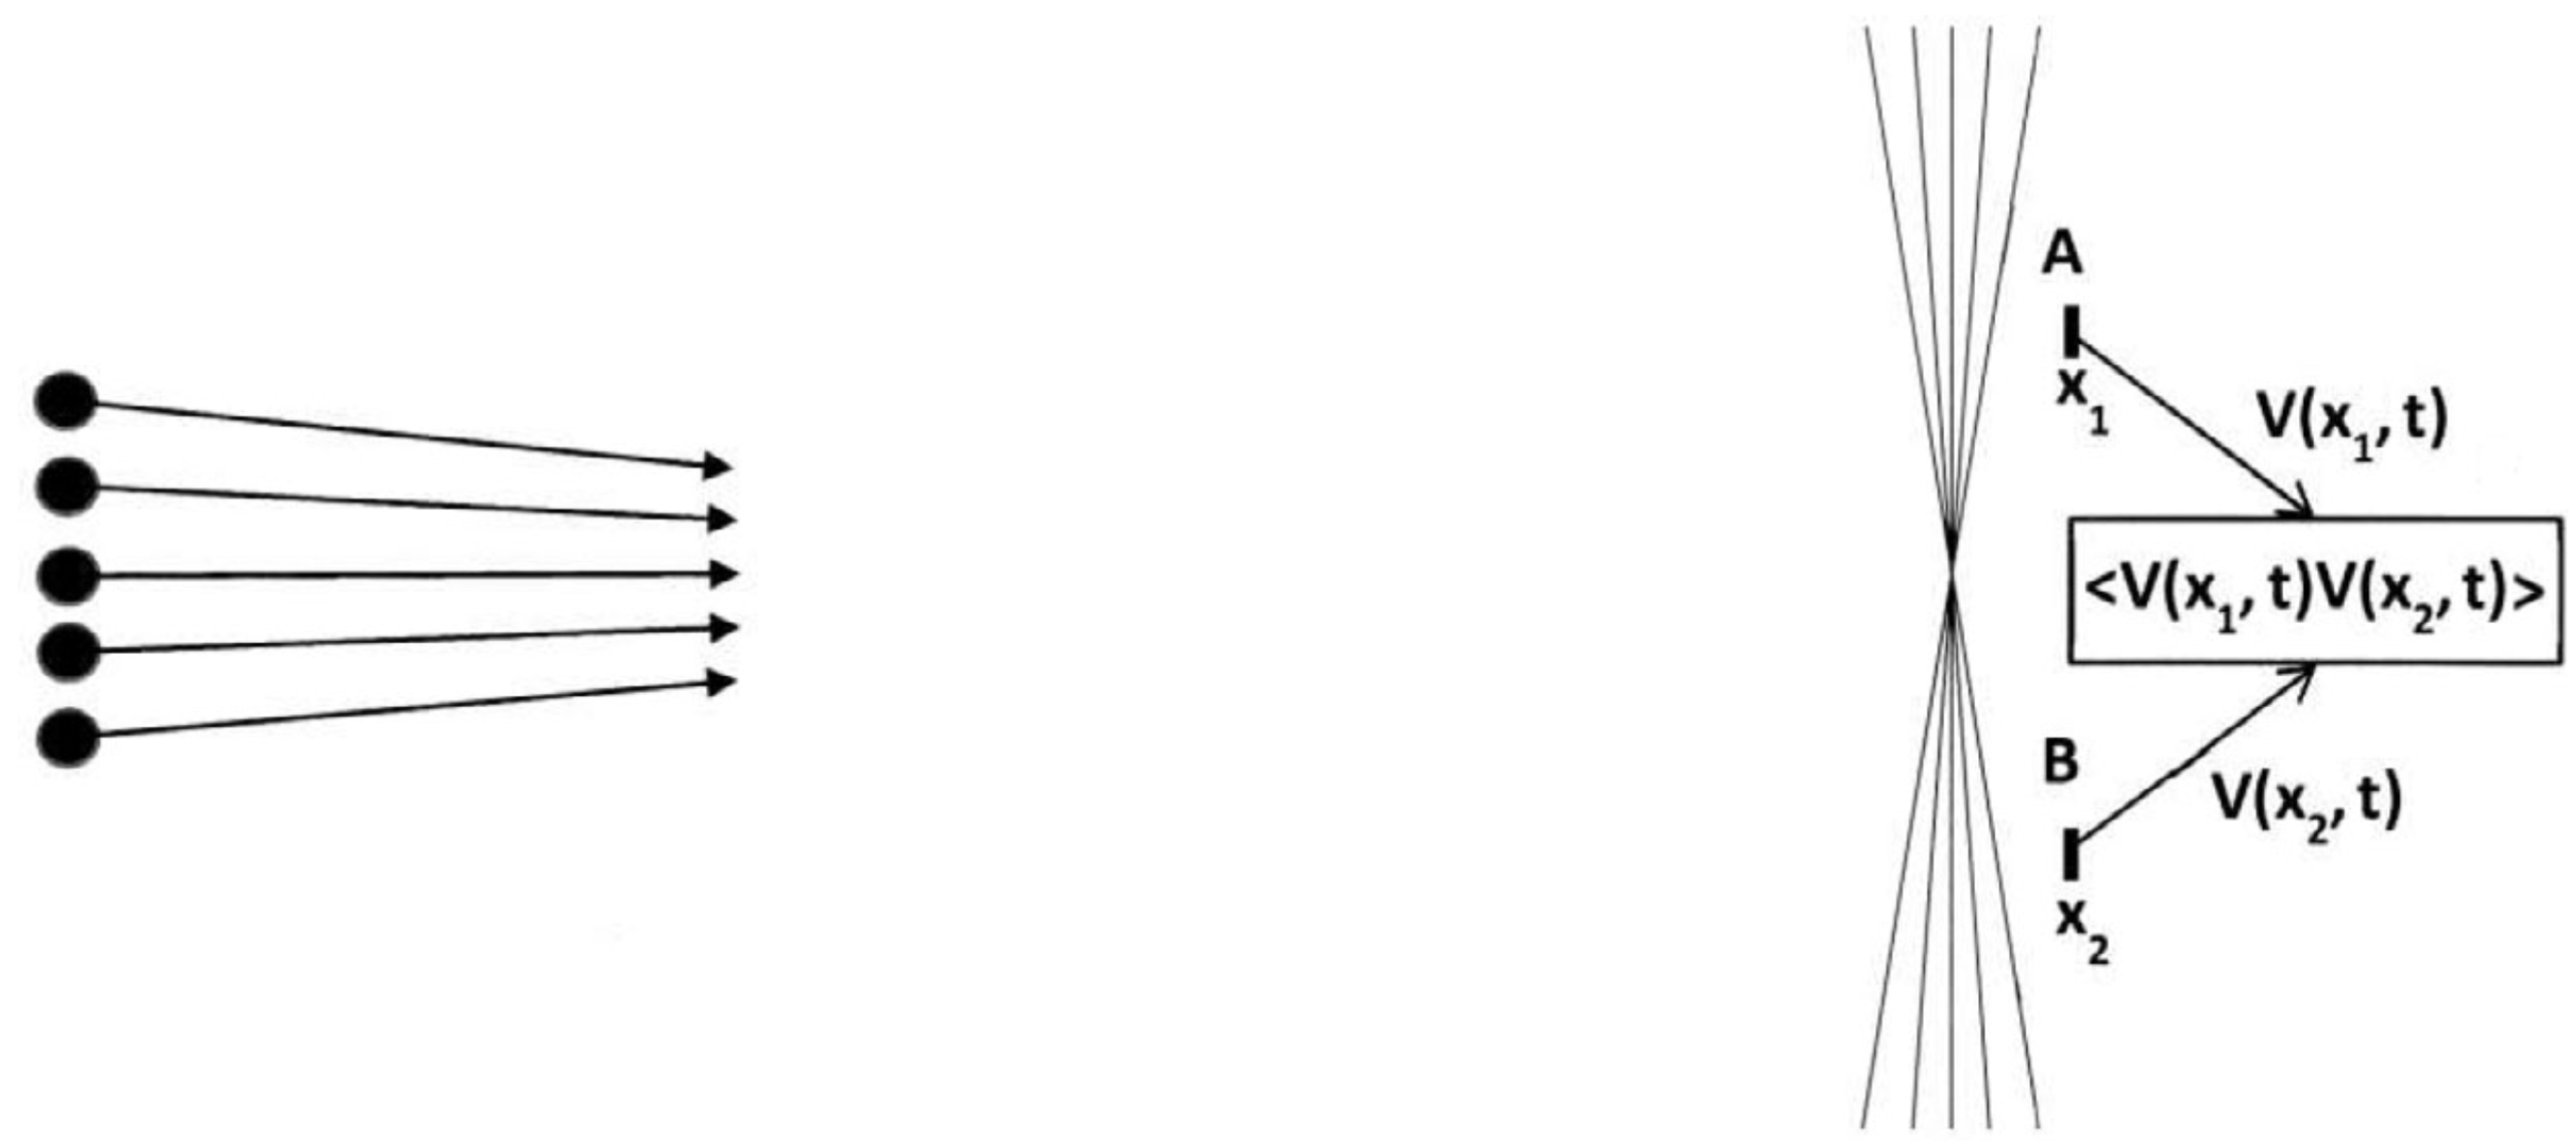
\includegraphics[width=0.8\textwidth]{images/Theorie/Burke_9.25.png}
    \caption{Abgebildet ist eine Skizze, die veranschaulicht, wie eine ausgedehnte inkohärente Quelle bei Teleskopseparationen $d>0$ trotzdem teilweise korreliertes Licht aufweist. Links ist eine Quelle schematisch in viele kohärente Punktquellen zerlegt, die ebene Wellen emittieren. In den beiden Detektoren rechts werden jeweils alle ebenen Wellen detektiert, allerdings kommen diese aufgrund der Geometrie zu leicht verschiedenen Zeiten an. Es ist deutlich, dass die Lichtfelder für steigende $d$ immer verschiedener werden (die Kohärenz sinkt), während sie für $d=0$ vollkommen identisch und somit kohärent sind. Die Abbildung ist \cite[Fig. 9.25]{burkeIntroductionRadioAstronomy2019} entnommen.}
    \label{fig:räumliche kohärenz einer ausgedehnten quelle}
\end{figure}
Diese Korrelation ist maximal für eine Teleskopseparation von $d=0$, da in diesem Fall in beiden Teleskopen exakt dasselbe Licht gemessen wird. 
Wird $d$ nun immer weiter erhöht, verringert sich die Korrelation zwischen den Feldern immer weiter. 
Die Lichtfelder bestehen aus immer verschiedeneren ebenen Wellen und sind sich weniger ähnlich. 
Ab einer Separation $d_0 \approx \Delta l_\mathrm{c}$ sind die Lichtfelder nicht mehr korreliert und $g^{(1)}$ fällt auf Null ab. 
Distanzen entlang der Ausbreitungsrichtung ($l_\mathrm{c}$) und transversal dazu $d_0$ werden im Michelson-Interferomter verknüpft, da die Lichtwellen von verschiedenen Orte zu einem Ort zusammengeführt werden müssen.
Dies schafft eine enge Verbindung zwischen transversaler (räumlicher) und longitudinaler (zeitlicher) Kohärenz.  
Für spektral breites Licht (wie für thermisches Licht von Sternen üblich) ist die Kohärenzlänge und damit die maximale Teleskopseparation sehr klein (vgl. \autoref{eq:tau(delta nu)}). 
Daher wird häufig auf entsprechend enge optische Filter zurückgegriffen, die die spektrale Breite des Lichts heruntersetzen, um die Kohärenzlänge zu erhöhen. \\


Messgröße des Michelson-Sterninterferometers ist im einfachsten Fall der Interferenzkontrast, definiert als \cite{foellmiIntensityInterferometrySecondorder2009}
\begin{equation}
    K = \frac{I_{\mathrm{max}}-I_{\mathrm{min}}}{I_{\mathrm{max}}+I_{\mathrm{min}}}=\left|g^{(1)}(\mathbf{r}, \bm{\rho}, t, \tau)\right|
\end{equation} 
Hierbei sind $I_{\mathrm{max}}$ bzw. $I_{\mathrm{min}}$ die Intensitätsmaxima bzw. -minima der gemessenen Intensität auf dem Schirm. 
$\tau$ ist hierbei die Zeitdifferenz zwischen den beiden Feldern, die durch die Strecke $d\cdot\sin \alpha$ in \autoref{fig:Michelson-Sterninterferometer} entsteht, und $\bm{\rho}$ der effektive Abstandsvektor zwischen den Teleskopen. 
Der effektive Teleskopabstand entspricht der Projektion des Teleskopabstandes $d$ in die Beobachtungsebene, die i. A. nicht parallel zu $d$ liegt. 
Durch komplexere Methoden lässt sich neben der Amplitude auch die Phase der komplexen Funktion $g^{(1)}(\mathbf{r}, \bm{\rho}, t, \tau)$ messen, vgl. dazu \cite[Kap. 4.3]{mandelOpticalCoherenceQuantum1995}. \\
Die Messung eines Sternendurchmessers lässt sich nun wie folgt bewerkstelligen:
Im Interferometer wird die Weglängendifferenz $d \cdot\sin \alpha$ durch die Wahl einer passenden Verzögerung kompensiert, sodass die Welle zwar an zwei verschiedenen Orten, aber effektiv zu ein und derselben Zeit gesampelt wird. 
$\tau=0$ und die Welle ist zeitlich kohärent \cite{foellmiIntensityInterferometrySecondorder2009}. 
Durch Messung des Interferenzkontrastes für verschiedene effektive Spiegelseparationen $\rho=|\bm{\rho}|$ lässt sich die räumliche Korrelationsfunktion erster Ordnung messen. 
Über das van Cittert-Zernike-Theorem lässt sich aus der gemessenen räumlichen Korrelationsfunktion nun über eine Fouriertransformation auf die Intensitätsverteilung der Quelle zurückschließen \cite[Gl. 4.4-40]{mandelOpticalCoherenceQuantum1995}:
\begin{equation}
    g^{(1)}(\bm{r}_1, \bm{r}_2) = \frac{\int_\sigma I(\bm{r}') \,\mathrm{e}^{-i\overline{k}\left(\bm{s}_2 - \bm{s}_1\right) \bm{r}'} d^2r'}{\int_\sigma I \left(\bm{r}'\right) d^2 r'}
    \label{eq:van Cittert-Zernike}
\end{equation}
Hierbei sind $\bm{r}_1=\bm{s}_1 r_1$ und $\bm{r}_2=\bm{s}_2 r_2$ die Verbindungsvektoren zwischen den Beobachtungsorten und einem Punkt der Quelle. 
Es erfolgt eine Integration der Intensität über alle Punkte der Quelle, d. h. alle $I\left(\bm{r}'\right)$ für alle $\bm{r}'\in \sigma$. 
$\overline{k}$ ist die durchschnittliche Wellenzahl des beobachteten Lichts an beiden Orten, d. h. $\overline{k} = \frac{2\pi\overline{\nu}}{c}$ mit der durchschnittlichen Frequenz $\overline{\nu}$ und der Ausbreitungsgeschwindigkeit $c$. 
Die erwähnten Größen sind zur Veranschaulichung ebenfalls in \autoref{fig:van Cittert-Zernike} skizziert. 
\begin{figure}[h]
    \centering
    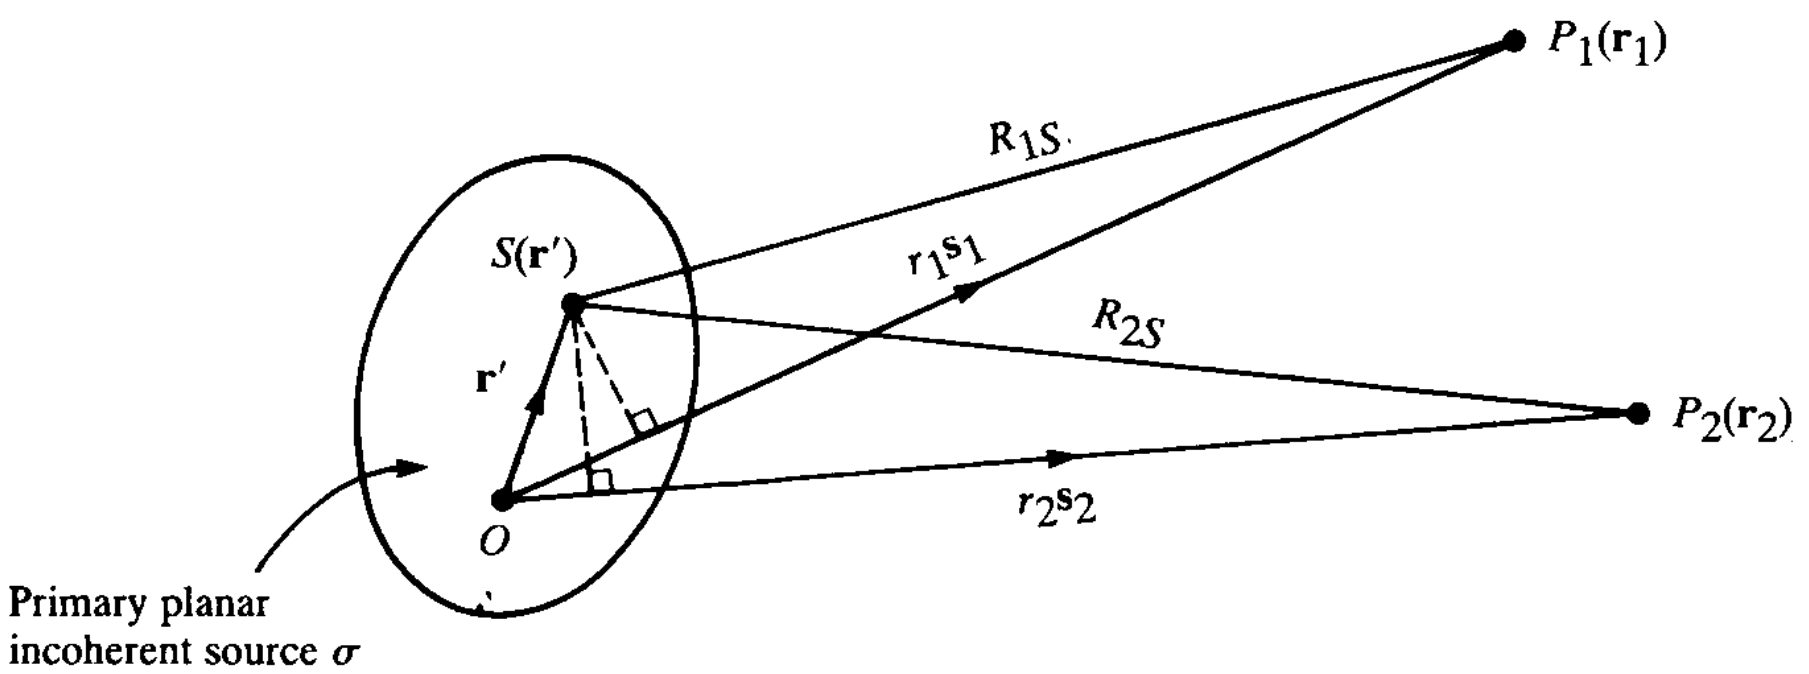
\includegraphics[width=0.8\textwidth]{images/Theorie/Mandel_4.12.png}
    \caption{Veranschaulichung der Größen aus \autoref{eq:van Cittert-Zernike}, entnommen aus \cite[Abb. 4.12]{mandelOpticalCoherenceQuantum1995}. Links ist die Quelle $\sigma$ zu sehen, während die Punkte $P_1$ und $P_2$ die Beobachtungsorte darstellen sollen. }
    \label{fig:van Cittert-Zernike}
\end{figure}
Der Vollständigkeit halber soll hier auch auf die Rolle der zeitlichen Korrelation $g^{(1)}(\tau)$ eingegangen werden. 
Diese stellt zwar bei interferometrischen Beobachtungen selten die primäre Observable dar, enthält aber trotzdem Informationen über die Quelle. 
Während die räumliche Korrelationsfunktion erster Ordnung mit dem Intensitätsprofil der Quelle zusammenhängt, gilt für $g^{(1)}(\tau)$ das Wiener-Khintchine-Theorem \cite{lasseguesFieldIntensityCorrelations2022}:
\begin{equation}
    S(\omega) =  \int g^{(1)}(\tau) e^{i\omega\tau} d\tau
\end{equation}
Das Spektrum der Quelle $S(\omega)$ ist die Fouriertransformierte der zeitlichen Korrelationsfunktion erster Ordnung. \\
Auch wenn wie erwähnt $g^{(1)}(\tau)$ häufig nicht die primäre Observable ist, soll hier noch einmal explizit erwähnt werden, dass für eine interferometrische Beobachtung nie \emph{nur} die räumliche Kohärenz der Quelle ausschlaggebend ist. 
Um nicht verschwindende räumliche Kohärenz messen zu können, muss $d\lesssim \Delta l_\mathrm{c}$ gelten, d. h. eine gewisse zeitliche Kohärenz vorherrschen. 
Nach \autoref{eq:tau(delta nu)} ist dies zu erreichen indem das Licht durch optische Filter spektral so verengt wird, dass ausreichend zeitliche Kohärenz vorliegt. 
Es ist ersichtlich, dass räumliche und zeitliche Kohärenz eng verknüpfte Konzepte darstellen, die lediglich in der Theorie klar getrennt sind. 
Daher ist es nicht verwunderlich, dass die Notwendigkeit spektraler Filter zur Herstellung zeitlicher Kohärenz auch bei der Einführung der Intensitätsinterferometrie in \autoref{ssec:Intensitätsinterferometrie} von Belang sein wird, obwohl die Begriffe Kohärenzzeit und -länge weniger klar deutbar sind. \\

Ein Nachteil des Michelson-Sterninterferometers ist die schwierig herzustellende Stabilität im Teleskop. 
Da die Wellen direkt miteinander interferieren, muss der Weg des Lichts auf einen Bruchteil einer Wellenlänge stabilisiert werden, um Phasenstabilität sicherzustellen. 
Dies wird insbesondere schwieriger, je größer die Spiegelabstände werden, was das Herstellen großer Winkelauflösungen erschwert. 
Weiterhin induzieren atmosphärische Variabilitäten schwer vorherzusagende Phasendifferenzen zwischen den beiden Teleskopen, die das Interferenzenmuster beeinflussen \cite[Kap. 2]{brownIntensityInterferometerIts1974}. 
Durch dieses sogenannte \glqq Seeing\grqq\;und die Notwendigkeit eines mechanisch sehr präzisen und stabilen Aufbaus sind Michelson-Sterninterferometer in ihrer Größe limitiert. 
Um beide Probleme zu umgehen, haben Hanbury Brown und Twiss ein modifiziertes System entwickelt -- das Intensitätsinterferometer.

\subsection{Intensitätsinterferometrie}
\label{ssec:Intensitätsinterferometrie}
Im Gegensatz zum Michelson-Sterninterferometer, in dem die Amplituden der Lichtwellen direkt zur Interferenz gebracht werden, werden im von Hanbury Brown und Twiss erstmals 1955 im Labor durchgeführten Experiment \cite{brownCorrelationPhotonsTwo1956} die Intensitäten direkt mit zwei Photomultipliern gemessen. 
Anschließend werden anstatt der Lichtwellen direkt die Photoströme miteinander korreliert. 
Bereits in den 1960ern und 70ern entwickelten Hanbury Brown und Twiss auf das erfolgreiche Laborexperiment und weitere Tests folgend das erste Intensitätsinterferometer, das \emph{Narrabi Stellar Intensity Interferometer} und bestimmten die Winkeldurchmesser von 32 Sternen \cite[Kap. 1]{brownIntensityInterferometerIts1974}. \\
Dies war nur möglich aufgrund des vergleichsweise einfachen Aufbaus. 
An beiden Teleskopen wird voneinander unabhängig der Photonenstrom, z. B. mittels Photomultipliern, gemessen und anschließend elektronisch korreliert. 
Vor- und Nachteil dieser Vorgehensweise ist die Insensitivität gegenüber Phasenunterschieden zwischen dem eintreffenden Licht an beiden Teleskopen. 
Einerseits geht durch die Messung Information (über die Phase) verloren, andererseits wird der Aufbau einfacher, da weder Phasenstabilität zwischen Teleskopen noch atmosphärisches Seeing einen Einfluss auf das korrelierte Signal haben.
Dieses Vorgehen ermöglicht im Prinzip beliebig lange Separationen und damit beliebig gute Winkelauflösungen. 
Vorraussetzung dafür ist lediglich, die Distanz zwischen Teleskopen im Vergleich zur Länge, die das Licht in der Detektorzeitauflösung zurücklegt, genau zu kennen \cite{DemonstrationStellarIntensity}. 
%So werden mit den VERITAS-Teleskopen z. B. mittels Intensitätsinterferometrie von Licht mit der Wellenlänge $\lambda_{\mathrm{eff}}=416\,\mathrm{nm}$ und effektiven, maximalen Teleskopseparationen von $r_{\mathrm{avg}}=157{,}9\,\mathrm{m}$ Winkelauflösungen von etwa $0{,}6\,\mathrm{marcsec}$ erreicht \cite{DemonstrationStellarIntensity}.
\\
Eine schematische Darstellung des Intensitätsinterferometers ist in \autoref{fig:Intensitätsinterferometer} dargestellt. 
\begin{figure}[h]
    \centering
    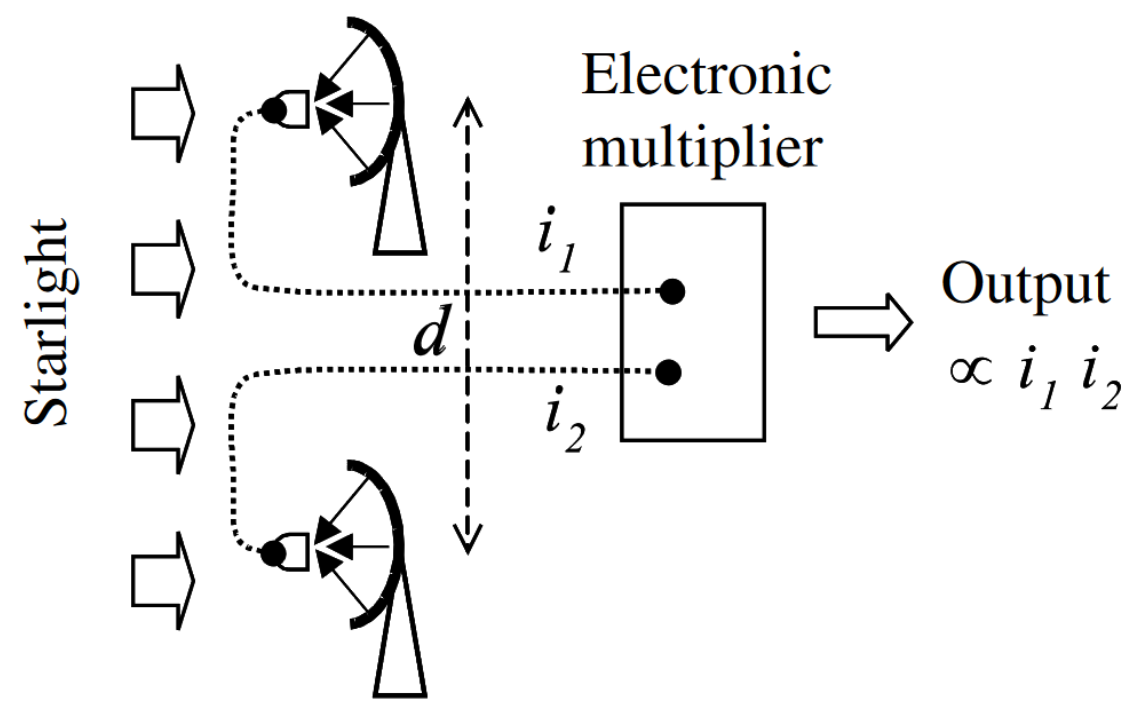
\includegraphics[width=0.65\textwidth]{images/Theorie/Fox_6.1b.png}
    \caption{Eine Skizze des Intensitätsinterferometers ist abgebildet. Das gesammelte Licht wird direkt detektiert und das zu den Intensitäten proportionale Signal elektronisch kombiniert. Entnommen aus \cite[Fig. 6.1(b)]{foxQuantumOpticsIntroduction2006}.}
    \label{fig:Intensitätsinterferometer}
\end{figure}
Zur Beschreibung der Korrelation von Intensitäten ist eine Erweiterung der bisher genannten Theorie nötig. 
Es bietet sich an, eine Korrelationsfunktion zweiter Ordnung einzuführen. 
Diese lässt sich erneut in relativen Abständen definieren, sodass $\bm{\rho} = \mathbf{r_2} - \mathbf{r_1}$ und $\tau = t_2 - t_1$, womit folgt (vgl. \cite{foellmiIntensityInterferometrySecondorder2009}):
\begin{equation}
    g^{(2)}(\mathbf{r}, t, \bm{\rho}, \tau) = \frac{\left<E^*(\mathbf{r}, t)E^*(\mathbf{r}+\bm{\rho}, t+\tau)E(\mathbf{r}+\bm{\rho}, t+\tau)E(\mathbf{r}, t)\right>}
        {\left<E^*(\mathbf{r}, t)E(\mathbf{r}, t)\right>^2}
\end{equation}
Mit der Notation $I=\left<I(t)\right>$ und unter der Annahme von thermischem, bzw. chaotischem Licht, in dem die Phasen der emittierten Lichtquanten zufällig verteilt sind, folgt:
\begin{equation}
    g^{(2)}(\mathbf{r}, \bm{\rho}, t, \tau) =  \frac{\left<I(\mathbf{r}, t) I(\mathbf{r}+\bm{\rho}, t+\tau)\right>}{I^2}
    \label{eq:g2_final}
\end{equation}
Durch das Interferometer kann nun (analog zu $g^{(1)}(\bm{\rho})$ beim Michelson-Sterninterferometer) $g^{(2)}(\bm{\rho})$ gemessen werden. 
Um nun trotzdem auf die Quellengeometrie schließen zu können, wird ein Zusammenhang zwischen $g^{(1)}$ und $g^{(2)}$, die sog. Siegert-Relation, genutzt \cite{lasseguesFieldIntensityCorrelations2022}:
\begin{equation}
    g^{(2)}(\tau) = 1+ \left|g^{(1)}(\tau)\right|^2
\end{equation}
Diese gilt nur für chaotisches und thermisches Licht. 
Unter chaotischem Licht versteht man Licht, dessen Quanten aufgrund von Stößen unter emittierenden Gasmolekülen und der Eigenbewegung dieser mit zufälliger Phase emittiert werden. 
Es weist ähnlich wie thermisches Licht, welches Schwarzkörperstrahlung entspricht, Intensitätsschwankungen auf der Zeitskala einer Kohärenzzeit auf. 
Ein Beispiel für thermisches Licht ist die Emission eines Sterns und ein Beispiel für chaotisches Licht das Licht einer Gasentladungslampe \cite{foxQuantumOpticsIntroduction2006}. \\
Über eine Messung von $g^{(2)}$ mit dem Intensitätsinterferometer kann also mit der Siegert-Relation auf $\left|g^{(1)}\right|$ geschlossen werden. 
Da die Phaseninformation von $g^{(1)}$ durch dieses Vorgehen unbekannt ist, kann nicht direkt durch Anwendung des van Cittert-Zernike-Theorems auf die Quellengeometrie geschlossen werden. 
Stattdessen wird üblicherweise ein Modell der Lichtquelle angenommen, von welchem die Fouriertransformation bekannt ist. 
Durch einen Fit dieser an die gemessenen Daten lassen sich abschließend physikalische Größen wie der Durchmesser der Quelle bestimmen. \\
Ein Beispiel für typische im Labor auftretende Größenordnungen der räumlichen Korrelationsfunktionen ist in \autoref{fig:g1(rho),g2(rho) für versch Lochblenden} dargestellt. 
Hierbei wird als \glqq Stern\grqq\;eine von einer chaotischen Lichtquelle uniform ausgeleuchtete Lochblende des Durchmessers $d$ im Abstand $x$ angenommen. 
Dies entspräche im einfachsten Sternmodell einer uniform leuchtenden Scheibe einem Stern mit Winkeldurchmesser $\Delta \theta = \frac{d}{x}$. 
Für dieses Modell gilt nach \cite[Kap. 4.1]{brownIntensityInterferometerIts1974}:
\begin{align}
    \left| g^{(1)}(\rho)\right| &= \frac{2J_1\left(\frac{\pi\rho\Delta\theta}{\lambda_0}\right)}{\frac{\pi\rho\Delta\theta}{\lambda_0}}\quad\quad\quad \Rightarrow & g^{(2)}(\rho) &= 1 + \left[\frac{2J_1\left(\frac{\pi\rho\Delta\theta}{\lambda_0}\right)}{\frac{\pi\rho\Delta\theta}{\lambda_0}}\right]^2
\end{align}
Hierbei sind $J_1$ die Besselfunktion erster Ordnung und $\lambda_0$ die zentrale Wellenlänge, gegeben durch den verwendeten Filter. 
Für Werte von $x=1{,}75\,\mathrm{m}$ und $\lambda_0=465\,\mathrm{nm}$ ergeben sich die in \autoref{fig:g1(rho),g2(rho) für versch Lochblenden} gezeigten Verläufe. 
\begin{figure}[h]
    \centering
    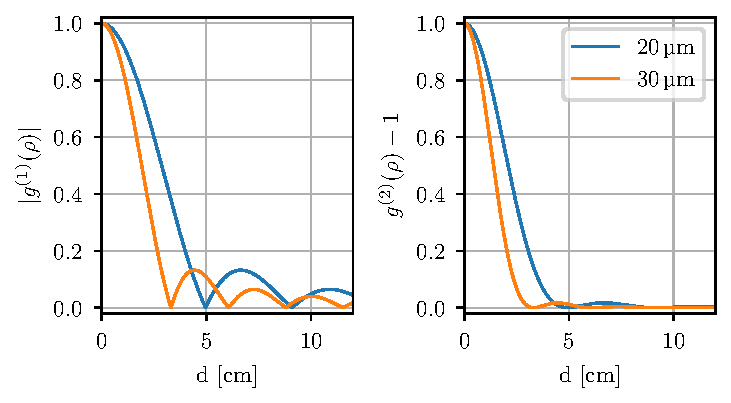
\includegraphics{images/Theorie/g1_g2_rho.pdf}
    \caption{Gezeigt sind die Verläufe von $g^{(1)}(\rho)$ und $g^{(2)}(\rho)$ für zwei Lochblenden mit Durchmesser $20\,\mathrm{\mu m}$ und $30\,\mathrm{\mu m}$. Für beide Lochblenden ist $x=1{,}75\,\mathrm{m}$ und $\lambda_0=465\,\mathrm{nm}$.}
    \label{fig:g1(rho),g2(rho) für versch Lochblenden}
\end{figure}
Durch Samplen der Funktion $g^{(2)}(\rho)$ kann die erste Nullstelle bestimmt werden, die für das genannte Modell bei 
\begin{equation}
    \rho_0=1{,}22\frac{\lambda_0}{\Delta\theta} 
    \label{eq:erste nulstelle von g2(rho) für lochblende}
\end{equation}
liegt \cite[Kap. 4.1]{brownIntensityInterferometerIts1974}. 
Aus dieser kann dann der Winkeldurchmesser berechnet werden. 
Es ist ersichtlich, dass typische Größenordungen von $\rho_0$ im Labor bei wenigen Zentimetern liegen, während bei Sternen Separationen im Bereich von hundert Metern bis zur ersten Nullstelle üblich sind (vgl. z. B. \cite[Abb. 10.2]{brownIntensityInterferometerIts1974}). \\


Um $g^{(2)}(\rho)$ für verschiedene effektive Teleskopseparationen zu samplen, wird für jede Distanz $\rho=|\bm{\rho}|$ die zeitliche Korrelationsfunktion zweiter Ordnung gemessen, indem die gemessenen Intensitäten miteinander korreliert werden. 
Deswegen soll im Folgenden der erwartete Verlauf der Observablen $g^{(2)}(\tau)$ näher beschrieben werden. 
Anhand des Verhaltens von $g^{(2)}(0)$ lassen sich drei Phänomene unterscheiden \cite{foxQuantumOpticsIntroduction2006}. 
\begin{itemize}
    \item $g^{(2)}(0)=1$: Die Photonen treffen mit zufälligen Abständen auf den Detektor. Das Licht ist kohärent und es gilt allgemein $g^{(2)}(\tau)=1$. Dies gilt für einen idealen, monochromatischen Laser \cite[Kap. 9]{mansuripurClassicalOpticsIts2009}.
    \item $g^{(2)}(0)>1$: Die Photonen erreichen die Detektoren gebündelt in sog. \emph{bunches}. Die Korrelation ist erhöht bei niedrigen Zeitdifferenzen. Mit anderen Worten ist es also wahrscheinlicher, ein weiteres Photon zu messen, wenn zuvor bereits eines gemessen wurde. Thermisches und chaotisches Licht zeigen Bunching.
    \item $g^{(2)}(0)<1$: Die Photonen treffen in regelmäßigen Abständen auf den Detektor. Es ist daher unwahrscheinlicher als im kohärenten Fall, kurz nach der Messung eines Photons ein weiteres zu messen. Dieses Phänomen bezeichnet man als Antibunching. 
\end{itemize}
Eine Veranschaulichung der Einteilung des Lichtes ist in \autoref{fig:bunching} gezeigt. 
\begin{figure}[h]
    \centering
    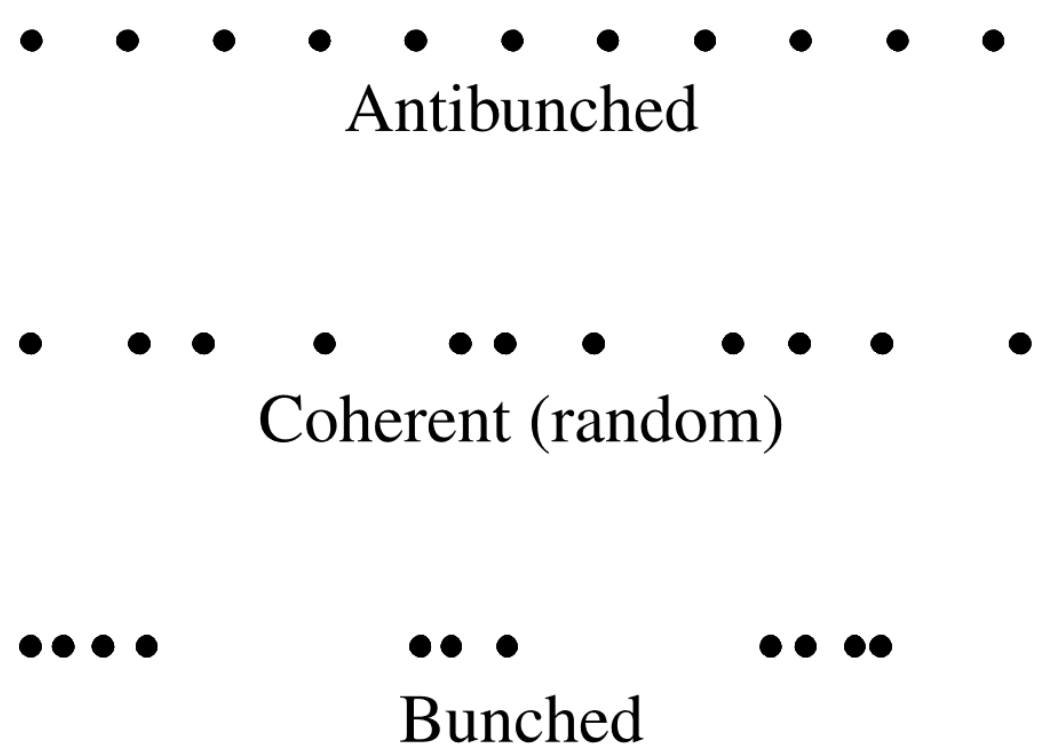
\includegraphics[width=0.4\textwidth]{images/Theorie/Fox_6.6.png}
    \caption{Anitbunching, kohärente Photonen und Bunching sind schematisch dargestellt. Während die Photonenabstände bei kohärentem Licht zufällig sind, sind bei Antibunching regelmäßige und bei Bunching geringe Abstände wahrscheinlicher. Abbildung aus \cite[Abb. 6.6]{foxQuantumOpticsIntroduction2006}}
    \label{fig:bunching}
\end{figure}
Eine weitere geläufige Einteilung des Lichts wird aufgrund der Photonenstatistik, also der Verteilung der gemessenen Einzelphotonen in einem gewissen Zeitintervall, vorgenommen. 
Nach dieser Einteilung ist die Anzahl gemessener kohärenter Photonen poissonverteilt, während gebunchte Photonen einer breiteren und antigebunchte Photonen einer schmaleren Verteilung folgen. 
Eine tiefergehende Beschreibung findet sich z. B. in \cite[Kap. 5.4-5.6]{foxQuantumOpticsIntroduction2006}. \\

Durch die Siegert-Relation und den bereits beschriebenen Verlauf von $g^{(1)}(\tau)$ lässt sich auf das Aussehen von $g^{(2)}(\tau)$ schließen (vgl. \cite[Kap. 6.3]{foxQuantumOpticsIntroduction2006}). 
So ist bei einem idealen Detektor $g^{(2)}(0)=2$ und fällt für $|\tau|>0$ immer weiter ab, bis sich $g^{(2)}$ nach einer Zeit in der Größenordnung der Kohärenzzeit, also für $\tau\gtrsim\tau_{\mathrm{c}}$, dem Wert 1 annähert. 
Da $g^{(2)}(\tau)$ bei chaotischen Lichtquellen wie bereits erwähnt über eine Fouriertransformation mit dem Spektrum der Quelle zusammenhängt, ergibt sich je nach verwendetem Filter ein anderer Verlauf von $g^{(2)}(\tau)$ zwischen dem Wert 2 und 1. 
Ein beispielhafter Verlauf von $g^{(1)}(\tau)$ und $g^{(2)}(\tau)$ ist in \autoref{fig:g1(tau),g2(tau) für versch Filter} für einen Filter mit rechteckigem Transmissionsprofil, zentraler Wellenlänge $\lambda_0 = 465\,\mathrm{nm}$ und Breiten $\Delta\lambda$ von 2\,nm und 5\,nm aufgezeigt. 
Für die normalisierte Fouriertransformation einer Rechteckfunktion $\mathrm{rect}_{\Delta f}\left(f\right)$ und damit $g^{(1)}(\tau)$ gilt (vgl. \cite[Kap. 3.2]{wangIntroductionOrthogonalTransforms2012}):
\begin{align}
    g^{(1)}(\tau) &= \mathrm{sinc}\left(\tau\Delta f\right) \quad\quad\quad \Rightarrow& g^{(2)}(\tau) &= 1+ \left[\mathrm{sinc}\left(\tau\Delta f\right)\right]^2
\end{align}
Hierbei entspricht $\Delta f$ der Umrechnung von $\Delta\lambda$ in den Frequenzraum, d. h. 
\begin{equation}
    \Delta f = \frac{c}{\lambda_0 - \nicefrac{\Delta\lambda}{2}} - \frac{c}{\lambda_0 + \nicefrac{\Delta\lambda}{2}}
\end{equation}
\begin{figure}[h]
    \centering
    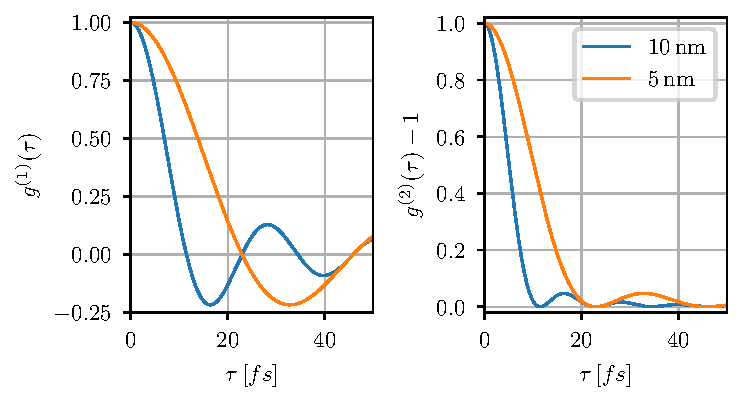
\includegraphics{images/Theorie/g1_g2_tau.pdf}
    \caption{Abgebildet ist der Theorieverlauf von $g^{(1)}(\tau)$ und $g^{(2)}(\tau)$ für einen Filter mit rechteckigem Transmissionsprofil mit Breite 2, bzw. 5\,nm, zentriert um 465\,nm.}
    \label{fig:g1(tau),g2(tau) für versch Filter}
\end{figure}
In einer realen Messung verringert das Binning der Messdaten in Intervalle $\tau_\mathrm{B}$ den Wert von $g^{(2)}(0)$ zusätzlich. 
Da dieses zumeist deutlich größer ist als die Kohärenzzeit, werden im zentralen Bin $\tau \in [0, \tau_\mathrm{B}]$ neben den kohärenten Photonen auch ein Faktor $\nicefrac{\tau_\mathrm{B}}{\tau_{\mathrm{c}}}$ mehr zufällig koinzidente Photonen gemessen. 
Dies verringert $g^{(2)}(0)$ um ebendiesen Faktor \cite[Kap. 14.7]{mandelOpticalCoherenceQuantum1995}. 
Weiterhin wird durch eine endliche Zeitauflösung des Detektors $g^{(2)}(0)$ weiterhin verringert, da kohärente Photonen auch außerhalb des zentralen Bins auftreten können und so nicht zu diesem beitragen. 
Dies verdeutlicht eine weitere Herausforderung in der angewandten Intensitätsinterferometrie. 
Da die Kohärenzzeit oft deutlich kürzer ist als die Zeitauflösung und das Binning, ist das zu messende Signal sehr klein, was ein geringes Signal-Rausch-Verhältnis zur Folge hat. 
Daher ist häufig eine lange Messzeit nötig, um die Form von $g^{(2)}(\tau)$ aus den verrauschten Messdaten extrahieren zu können. \\
Eine weitere Folge der vergleichsweise geringen Zeitauflösung ist, dass sich $g^{(2)}(\rho, \tau=0)$ nicht gezielt messen lässt. 
Stattdessen misst man effektiv $g^{(2)}(\rho, \tau\in(-\infty, \infty))$. 
Es ergibt also Sinn, $\tau_{\mathrm{c}}$ als ebendieses Integral zu definieren \cite[Eq. 14.7-2]{mandelOpticalCoherenceQuantum1995}: 
\begin{equation}
    \tau_{\mathrm{c}} := \int_{-\infty}^{\infty} \left|g^{(1)}(\tau) \right|^2\;d\tau = \int_{-\infty}^{\infty} \left(g^{(2)}(\tau) - 1\right)\;d\tau
\end{equation}
Zur Messung von Sternendurchmessern wird mit dieser Vorgehensweise also für jede Teleskopseparation $\rho$ die Funktion $g^{(2)}(\tau)$ gemessen und integriert, um $\tau_{\mathrm{c}}$ zu bestimmen. 
Da gilt $\tau_{\mathrm{c}}(\rho)\propto g^{(2)}(\rho)$ lässt sich abschließend wie in \autoref{fig:g1(rho),g2(rho) für versch Lochblenden} gezeigt auf $\Delta\theta$ schließen. \\

Abschließend soll noch gezeigt werden, dass ein Einfluss der Kabellänge auf $g^{(2)}$ in der Theorie nicht erwartet wird. 
\autoref{eq:g2_final} folgend ergibt sich für die gemessene Korrelation zweier Photoströme $J_1(t)$ bzw. $J_2(t)$ und ihrem zeitlichen Mittelwert $J_1$ bzw. $J_2$:
\begin{equation}
    g^{(2)}(\tau) = \frac{\left<J_1(t) J_2(t+\tau) \right>}{J_1 J_2}
\end{equation}
Führt man nun eine zeitunabhängige Dämpfung der Signale um Faktoren $\alpha$ bzw. $\beta$ ein, wie diese durch unterschiedlich lange Koaxialkabel hervorgerufen werden würden, so folgt aufgrund der angenommenen Zeitunabhängigkeit:
\begin{equation}
    g^{(2)}(\tau)_{\mathrm{damp}} = \frac{\left<\alpha J_1(t) \beta J_2(t+\tau) \right>}{\alpha J_1 \beta J_2}
    = \frac{\alpha \beta}{\alpha \beta} \frac{\left<J_1(t) J_2(t+\tau) \right>}{J_1 J_2} = g^{(2)}(\tau)
\end{equation}
Es wird also kein Einfluss einer zeitunabhängigen Dämpfung auf den Wert von $g^{(2)}(\tau)$ und damit auf $\tau_{\mathrm{c}}$ erwartet. 
Da dieser aber in bisherigen Messungen der Arbeitsgruppe (z. B. \cite{zmijaFirstIntensityInterferometry2023}) trotzdem beobachtet wird, ist Ziel der nun folgenden Arbeit, diesen Effekt durch statistisch aussagekräftigere Labormessungen zu untersuchen. 
\clearpage
\mbox{}
\clearpage

\section{Aufbau und Erwartung an die Messergebnisse}
\label{sec:Aufbau}
Im Folgenden soll auf den verwendeten experimentellen Aufbau eingegangen werden. 
Dafür wird dieser zuerst anhand einer Skizze erklärt. 
Anschließend wird die bereits entwickelte Theorie auf den Aufbau bezogen und aufgezeigt, welche Abweichungen sich von der idealisierten Herangehensweise im vorangegangenen Abschnitt ergeben. 
In diesem Zuge wird abschließend die Erwartung an die Messgröße $\tau_{\mathrm{c}}$ berechnet, auf welche sich in späteren Abschnitten bezogen werden soll. \\

Am besten lässt sich der Versuchsaufbau anhand einer vereinfachten Skizze nachvollziehen. Diese ist daher in \autoref{fig:Versuchsaufbau} dargestellt. 
\begin{figure}[h]
    \centering
    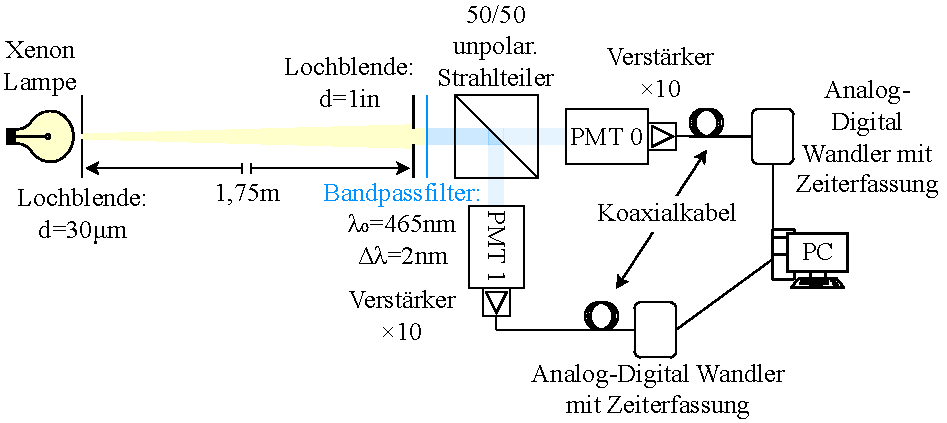
\includegraphics[width=0.9\linewidth]{images/Aufbau/Aufbau.pdf}
    \caption{Gezeigt ist eine vereinfachte Skizze des verwendeten Aufbaus, welche die konzeptuell wichtigsten Bestandteile darstellt.}
    \label{fig:Versuchsaufbau}
\end{figure}
Als Lichtquelle wird eine Xenonlampe (Osram XBO 75 W/2 \cite{XBO75OSRAM}) gewählt. 
Als Gasentladungslampe emittiert diese nach \autoref{ssec:Intensitätsinterferometrie} chaotisches Licht, welches Bunching aufweist. 
Da nach dem van Cittert-Zernike-Theorem der Winkeldurchmesser der Lichtquelle invers proportional zur Breite von $g^{(2)}(\bm{\rho})$ ist, ist weiterhin darauf zu achten, die Ausdehnung der Lichtquelle einzuschränken, damit korrelierte Photonen am Detektor vorliegen. 
Zu diesem Zweck ist eine kreisförmige Lochblende mit einem Durchmesser von $d=30\,\mathrm{\mu m}$ verbaut. 
Mit der Distanz $x=1{,}75\,\mathrm{m}$ zwischen Lichtquelle und dem restlichen Aufbau ergibt sich so ein Winkeldurchmesser von $\Delta \theta \approx \frac{d}{x} = 3{,}53\,\mathrm{arcsec}$. 
Es sei darauf hingewiesen, dass typische Winkeldurchmesser von Sternen im Bereich von tausendstel Bogensekunden liegen \cite{hanburybrownAngularDiameters321974}, also etwa drei Größenordnungen kleiner sind, als der hier geschaffene \glqq künstliche Stern\grqq. \\
Um dem eintretenden Lichtstrahl eine definierte Breite zu geben, wird dieser zusätzlich durch eine Lochblende mit einem Durchmesser von einem Zoll geleitet. 
Weiterhin wird das einfallende Licht so auf einen Bereich beschränkt, der etwa der effektiven Größe der Photomultiplier von $23\times 23\,\mathrm{mm}$ entspricht \cite{PhotomultiplierTubeR11265U200}. \\
Wie in \autoref{ssec:Michelson-Sterninterferometer} beschrieben, ist für eine Messung der räumlichen Kohärenz auch eine nicht verschwindende Kohärenzzeit relevant. 
Da diese indirekt proportional zur spektralen Breite der Quelle ist, wird an dieser Stelle ein enger Bandpassfilter (Alluxa 465-2 \cite{4652OD4Ultra}) mit einer annähernd rechteckförmigen Transmissivität verbaut. 
Dieser hat nach Herstellerangaben eine zentrale Wellenlänge von $\lambda_0 = 465\,\mathrm{nm}$ und eine Halbwertsbreite von  $\Delta\lambda = 2\,\mathrm{nm}$. 
Anschließend wird der Strahl durch einen nicht polarisierenden 50/50 Strahlteilerwürfel (Thorlabs BS031 \cite{ThorlabsBS03150}) aufgeteilt und zum Nachweis der Photonen auf zwei Photomultiplier (PMTs, Hamamatsu R11265U-200 \cite{PhotomultiplierTubeR11265U200}) gelenkt. 
Um bei hohen Photonenraten weiterhin eine lineare Verstärkung durch die PMTs zu erhalten, werden die letzten vier Dynoden mit einer Stabilisationsspannung betrieben \cite{zmijaOpticalIntensityInterferometry2021}. 
Als Spannungsquelle für die Hochspannung und die Stabilisationsspannung wird eine durch den Computer steuerbare Spannungsquelle (CAEN DT5533E \cite{DT5533E}) genutzt. 
Direkt am Ausgang der Photomultiplier werden die Pulse mit einem Verstärker (FAST ComTec TA1000B-10 \cite{TA1000BTimingAmplifier}) um den Faktor 10 verstärkt. 
Die Verstärkung direkt an den PMTs hat den Vorteil, dass Störsignale nicht vor der Verstärkung einkoppeln können, was das Signal-Rausch-Verhältnis verbessert. 
Anschließend werden die Signale durch variable Kombinationen an Kabellänge und -modell zu Analog-Digital-Wandlern (Spectrum M4I.2212-X8 \cite{M4i2212x8Bit} und Spectrum M4I.2211-X8 \cite{M4i2211x8Bit}, gleiches Modell, lediglich unterschiedlich viele Eingangskanäle) geleitet, wo diese digitalisiert werden. 
Obwohl die Spektrum-Karten vier bzw. zwei Digitalisierungskanäle unterstützen, werden zwei verschiedene und räumlich getrennte Karten genutzt, um ein Übersprechen zwischen den Kanälen zu verhindern. 
Aufgrund des von Natur aus geringen Signals werden alle analogen Signale durch geschirmte Koaxialkabel geleitet, um das Einkoppeln von Störsignalen zu erschweren. 
Um zusätzlich das Einkoppeln von störendem Licht des PCs oder sonstiger LEDs der Messgeräte zu erschweren, ist der optische Aufbau zudem durch ein Thorlabs-Röhrensystem fest verbunden, sodass nur Licht entlang der optischen Achse eindringen kann. 
Die zeitliche Synchronisierung der beiden des PMT-Strom-Verläufe (Waveforms) zur späteren Korrelation erfolgt durch Verwendung des White Rabbit Systems (vgl. z. B. \cite{lipinskiWhiteRabbitPTP2011}), welches direkt mit den Analog-Digital-Wandlern (ADCs) verbunden ist. 
Abschließend werden die Daten auf RAIDs (Areca ARC-8050T3U-12 \cite{ARC8050T3UThunderboltUSB}) zur späteren Korrelation gespeichert. \\
Da ein Ziel dieser Arbeit ist, zu untersuchen, wie sich verschiedene Kabel auf das Integral des Bunching Peaks auswirken, soll an dieser Stelle explizit auf die verwendeten Koaxialkabel eingegangen werden. 
Die ersten durchgeführten Messungen erfolgen mit 10 und 40\,m langen Kabeln des Typs Airborne 5 \cite{s.r.lAirborne10Coaxial}. 
Dies entspricht den Kabeln, welche in der von der Arbeitsgruppe 2022 durchgeführten Kampagne mit den H.E.S.S.-Teleskopen genutzt wurden \cite{zmijaFirstIntensityInterferometry2023}. 
Anschließend wurden noch Messungen mit Kabeln des Typs LMR 400 durchgeführt \cite{LMR400CoaxCable}. 
Diese weisen eine geringere Dämpfung auf als die Airborne 5 Kabel und sind daher interessant, um den Einfluss der Dämpfung auf das gemessene $\tau_{\mathrm{c}}$ zu untersuchen. \\

Aufgrund des speziellen Aufbaus ergeben sich einige Änderungen bezüglich der im vorangegangenen Abschnitt eingeführten Theorie. 
Auf diese soll hier eingegangen werden. 
Wie erwähnt ist der Winkeldurchmesser der Quelle vergleichsweise groß. 
Nach \autoref{eq:erste nulstelle von g2(rho) für lochblende} wird für die Distanz zur ersten Nullstelle der $g^{(2)}$-Funktion lediglich $\rho_0\approx3{,}3\,\mathrm{cm}$ erwartet. 
Das heißt, dass am Beobachtungsort lediglich zwischen Punkten, die maximal $\rho_0$ voneinander entfernt sind, korrelierte Photonen auftreten. 
Aufgrund der physischen Größe der PMTs ist es daher nicht möglich, $g^{(2)}(\rho)$ für verschiedene $\rho$ zu messen. 
Stattdessen wird ein Mittelwert von $g^{(2)}$ in einem Intervall von $\rho\in[0,1]$ Zoll gemessen. 
Dieses Intervall entspricht den Abständen, die korrelierte Photonen durch die Lochblende am Eingang des Strahlteilers haben können. 
Es wird also erwartet, einen niedrigeren Wert für $g^{(2)}(\rho)$ und damit $\tau_{\mathrm{c}}$ zu messen. 
Dies ist in \autoref{fig:räumliche koh simulation} verdeutlicht. 
Um herauszufinden, um welchen Faktor die gemessene Amplitude von der theoretischen maximalen Amplitude abweicht, wird eine von der Arbeitsgruppe geschriebene Simulation durchgeführt, die sowohl den Wert von $g^{(2)}$ für jeden Photonenabstand als auch die Wahrscheinlichkeit für diesen berücksichtigt. 
Der Faktor, um welchen $g^{(2)}$ im Vergleich zu $g^{(2)}(0)$ verringert ist, beträgt bei gegebenem Aufbau $k_\mathrm{T}=0{,}62$. 
Über den theoretischen Verlauf der Korrelationsfunktion lässt sich durch $k_\mathrm{T}$ auf einen effektiven Teleskopabstand $\rho\prime$ schließen, bei dem ein dünner Strahl denselben Verlust an räumlicher Kohärenz aufweist. 
Dies ist auch in \autoref{fig:räumliche koh simulation} veranschaulicht. 
\begin{figure}[ht]
    \centering
    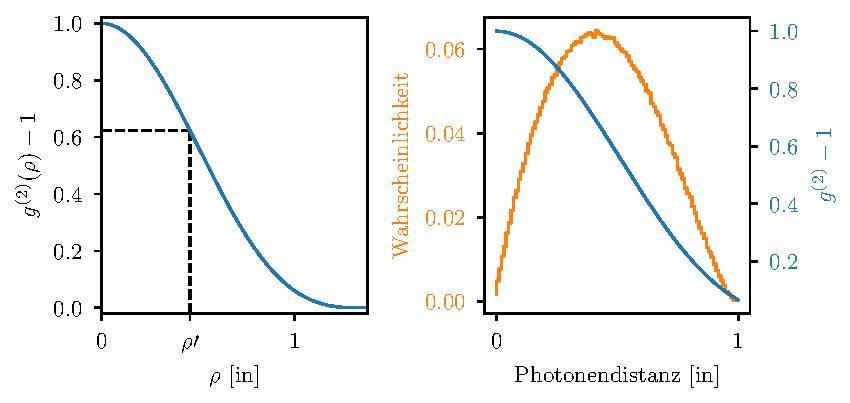
\includegraphics{images/Aufbau/g2(rho).pdf}
    \caption{Dargestellt ist links die $g^{(2)}$-Funktion, abhängig von der Separation $\rho$. Rechts ist das Ergebnis der Simulation abgebildet. In Blau ist $g^{(2)}$ für jeden Photonenabstand dargestellt (dies entspricht der Kurve im linken Graphen), während in Orange die simulierte Wahrscheinlichkeitsverteilung, ein Photonenpaar bei gegebenem Abstand anzutreffen, aufgetragen ist. Durch Multiplikation der beiden Kurven erhält man den Faktor, wie viel räumliche Kohärenz im Vergleich zum Maximum noch vorhanden ist. Dieser beträgt $k_\mathrm{T}=0{,}62$. Links ist zudem eingezeichnet, welchem Abstand $\rho\prime$ diese Kohärenz entsprechen würde. }
    \label{fig:räumliche koh simulation}
\end{figure}

Aus voriger Überlegung ist nun bekannt $\tau_{\mathrm{c}}^{\mathrm{expect}} = k_\mathrm{T}\cdot\tau_{\mathrm{c}}^{\mathrm{th}}$. 
Um den Theoriewert bei perfekter räumlicher Kohärenz $\tau_{\mathrm{c}}^{\mathrm{th}}$ zu bestimmen, wird eine weitere Simulation von der Arbeitsgruppe verwendet. 
Diese berechnet aus dem vom Hersteller gegebenen Transmissionspektrum des Filters über das Wiener-Khintchine-Theorem, d. h. eine Fouriertransformation, die erwartete $g^{(1)}$-Funktion, welche anschließend über die Siegert-Relation in $g^{(2)}(\tau, \rho=0)$ umgerechnet wird. 
Daraus folgt dann für den vorliegenden Fall $\tau_{\mathrm{c}}^{\mathrm{th}} = \int \left(g^{(2)}(\tau, \rho=0) -1\right) d\tau = 0{,}152\,\mathrm{ps}$. 
Abschließend ergibt sich also für die erwartete Kohärenzzeit bei verwendetem Aufbau:
\begin{equation}
    \tau_{\mathrm{c}}^{\mathrm{expect}} = 0{,}62 \cdot 0{,}152\,\mathrm{ps} = 94\,\mathrm{fs}
    \label{eq:tau_c_th}
\end{equation}

Da in den Faktor $k_\mathrm{T}$ der Winkeldurchmesser der Quelle und damit auch der Durchmesser der Lochblende nach der Xenonlampe eingeht und diese starker Hitze ausgesetzt ist, wurde zudem überprüft, ob die Herstellerangaben von 30\,$\mathrm{\mu m}$ noch zutreffen. 
Eine Aufnahme der Lochblende unter dem Mikroskop ist dafür in \autoref{fig:lochblende mikroskop} gezeigt. 
\begin{figure}[h]
    \centering
    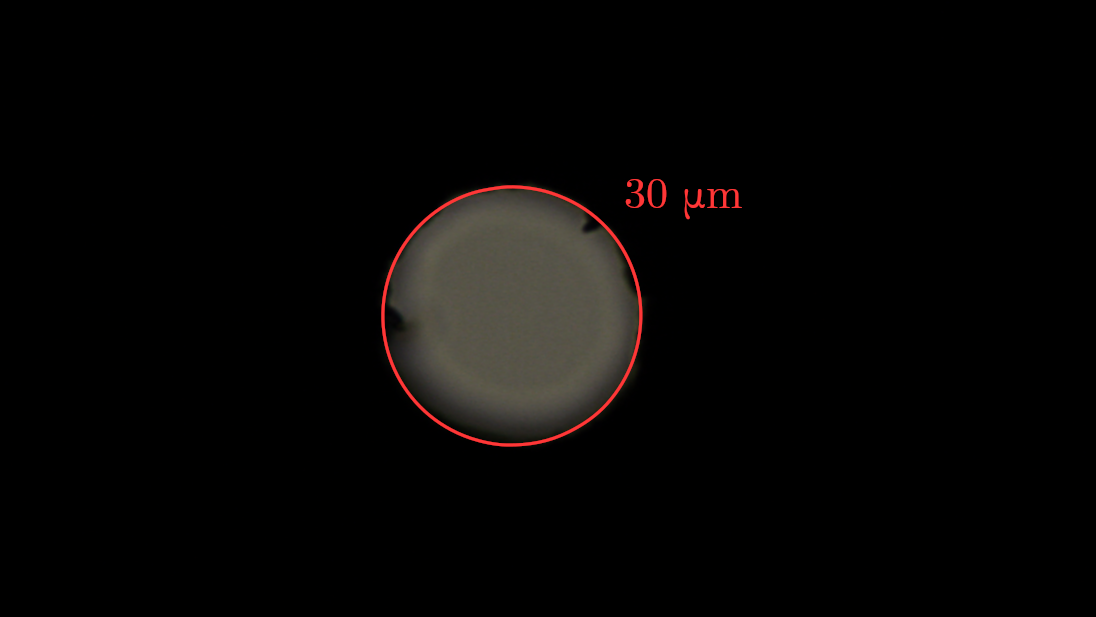
\includegraphics[width=0.8\textwidth]{images/Aufbau/Lochblende_Mikroskop.png}
    \caption{Die Mikroskopaufnahme der Lochblende sowie ein Kreis mit $30\,\mathrm{\mu m}$-Durchmesser sind gezeigt. Trotz irregulärer Strukturen am Rand entspricht der gemessene Durchmesser recht genau den Herstellerangaben.}
    \label{fig:lochblende mikroskop}
\end{figure}
Der eingezeichnete Kreis entspricht einem Durchmesser von $30\,\mathrm{\mu m}$. 
Auch wenn deutliche Abnutzungserscheinungen an den Rändern sichtbar sind, ist der gemessene Durchmesser sehr nah an den $30\,\mathrm{\mu m}$, die in die Berechnung von $k_\mathrm{T}$ eingehen. 
Der erwähnte Wert von $\tau_{\mathrm{c}}^{\mathrm{expect}}$ entspricht daher der Erwartung an die Messung und muss nicht noch zusätzlich wegen eines abweichenden Lochblendendurchmessers angepasst werden. 

\clearpage
\mbox{}
\clearpage

\section{Datenaufnahme und Pre-Processing}
\label{sec:Datenaufnahme und Pre-Processing}
In diesem Abschnitt soll auf die Datenaufnahme sowie alle nötigen Schritte der Datenverarbeitung bis zur fertigen $g^{(2)}(\tau)$-Funktion eingegangen werden. 
Dafür werden zuerst die Datenaufnahme und dafür nötige Kalibrationsverfahren erläutert. 
In diesem Zuge wird zudem auf das Aussehen der aufgenommenen Daten (Waveforms) eingegangen. 
Anschließend werden korrelierte Einzeldateien betrachtet und es wird verdeutlicht, warum eine Mittelung vieler Waveforms unumgäglich ist. 
Zuletzt werden angewandte Korrekturen und Filter angesprochen sowie verdeutlicht, wie die Mittelung der Daten erfolgt. 

\subsection{Datenaufnahme und Waveforms}
\label{ssec:Datenaufnahme und Waveforms}
Die Aufnahme der Daten erfolgt durch ein von der Arbeitsgruppe geschriebenes Programm, welches mit den ADCs kommuniziert. Ein Screenshot der GUI, auf dem die wichtigsten Schritte der Datenaufnahme markiert sind, ist in \autoref{fig:Screenshot GUI} eingefügt. 
\begin{figure}[h]
    \centering
    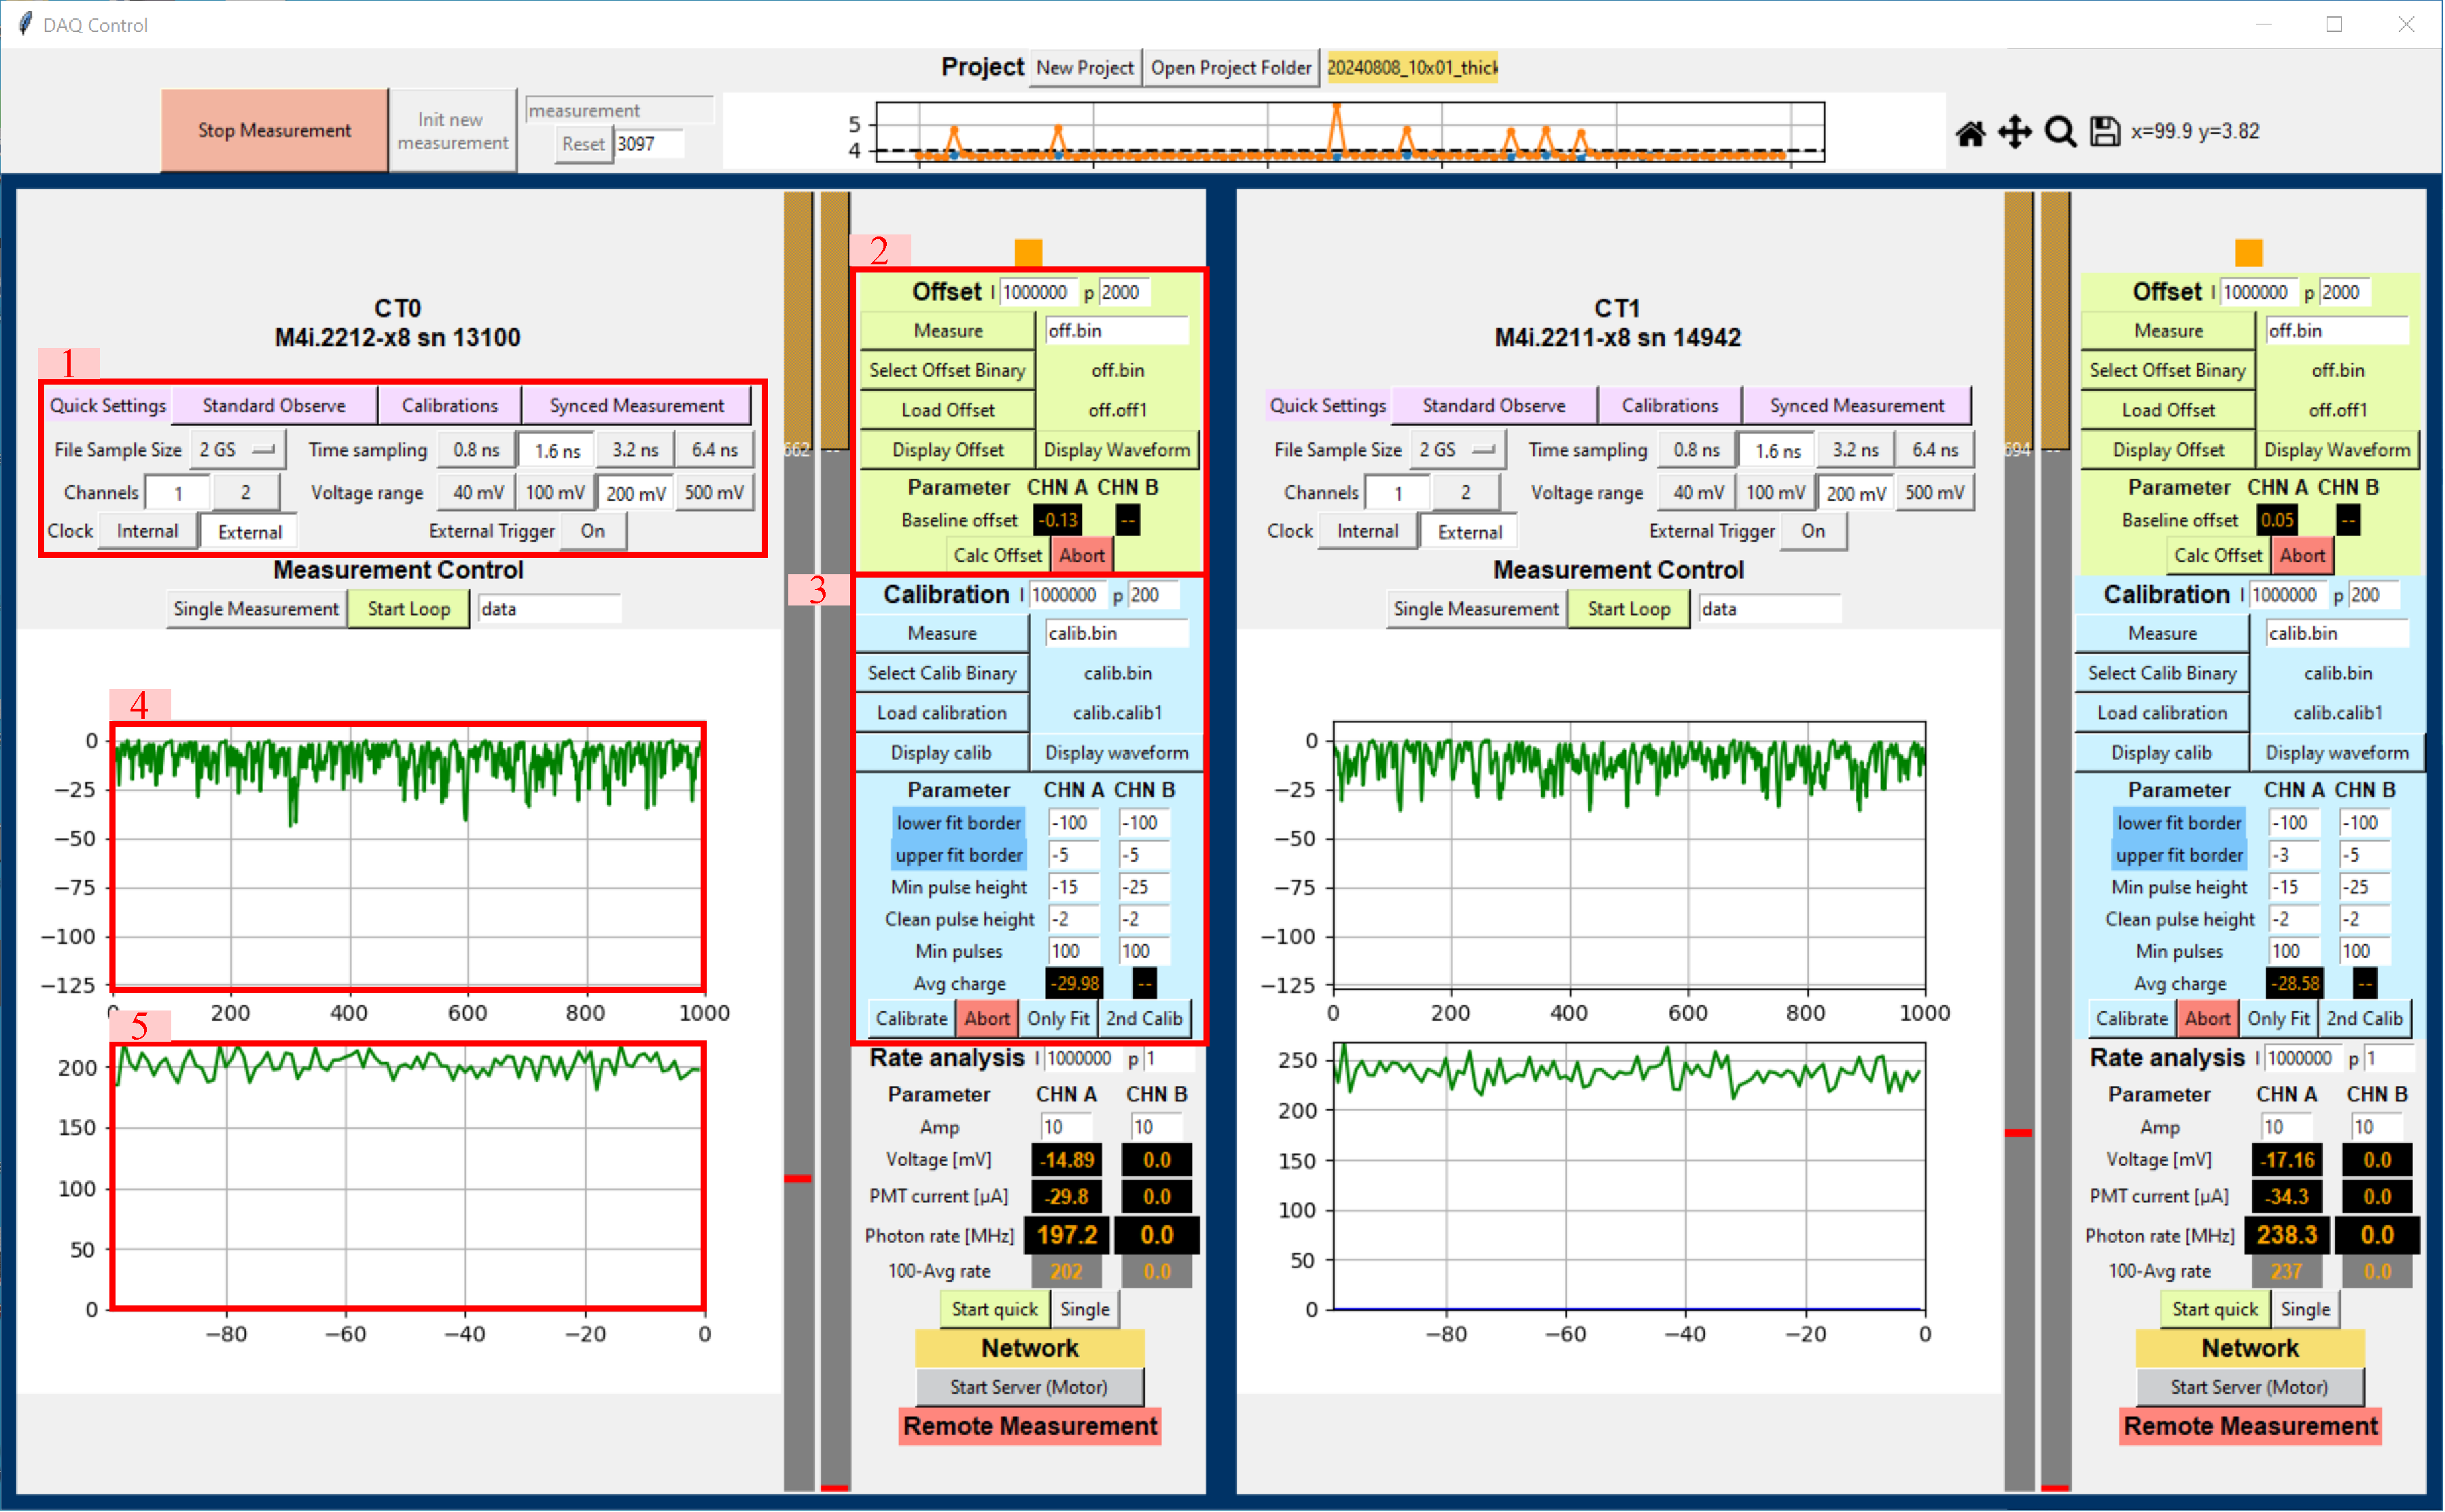
\includegraphics[width=0.9\textwidth]{images/Datenaufnahme/GUI.pdf}
    \caption{Dargestellt ist ein Screenshot der GUI zur Datenaufnahme. Wichtige Schritte sind markiert.}
    \label{fig:Screenshot GUI}
\end{figure}
In der GUI wird für jede verwendete Digitalisierungskarte ein Fenster erstellt, in dem Einstellungen für die jeweilige Karte vorgenommen werden können. 
Nach dem Erstellen eines Projekts können in dem mit \emph{1} markierten Bereich in \autoref{fig:Screenshot GUI} Einstellungen für die ADC-Karte vorgenommen werden. 
Es wird mit einem Kanal je Karte gemessen und die Samplingzeit beträgt $1{,}6$\,ns bei einer Dateigröße von 2 Gigasamplen. 
Der zu digitalisierende Spannungsbereich wird passend zu den in \emph{4} abgebildeten Waveforms auf 200\,mV gesetzt. 
Clock und Trigger werden extern durch das White Rabbit System gegeben. 
Die genannten Einstellung werden größtenteils vor der Messung automatisch mit dem Button \glqq Init new measurement\grqq\;gesetzt. \\
Vor Start der Messung müssen zwei Kalibrationsschritte für jeden Kanal gemacht werden. 
Zuerst wird unter \emph{2} eine Offset-Kalibration durchgeführt, indem \glqq Measure\grqq\;und \glqq Calc Offset\grqq\;gewählt werden. 
Diese wird ohne Beleuchtung und mit ausgeschalteter Hochspannung durchgeführt. 
Das Programm bestimmt diesen vom PMT abhängigen Offset und entfernt diesen, sodass dieser die Korrelation nicht beeinflusst \cite{zmijaOpticalIntensityInterferometry2021}. 
Anschließend wird bei eingeschalteter Hochspannung und niedriger Photonenrate eine Raten-Kalibration durchgeführt, sodass gemessene Spannungen in Photonenraten umgerechnet werden können. 
Dies ist nötig, da aufgrund der hohen Raten bei der Messung nicht Einzelphotonepulse, sondern ganze Waveforms miteinander korreliert werden. 
Für die Kalibration wird für jeden Kanal die mittlere Pulsform der PMT-Pulse bestimmt und gespeichert. 
Es wird erwartet, dass diese einen bedeutenden Einfluss auf die Form der $g^{(2)}$-Funktion hat, da die Photonenpulse deutlich breiter sind als die einzelnen $1{,}6$\,ns-Bins, was zu einer Korrelation benachbarter Bins führt \cite{zmijaOpticalIntensityInterferometry2021}. 
Aus den gemessenen Daten wird bestimmt, wie viel Ladung ein Photon, das auf einen PMT trifft, durchschnittlich freisetzt, woraus anschließend die in \emph{5} gezeigten Photonenraten in MHz bestimmt werden können. \\
Nach diesen Kalibrationsschritten kann die Messung gestartet werden, woraufhin synchronisiert durch den Trigger des White Rabbit Systems 2$\cross$2\,GS Daten aufgenommen werden. 
Dies entspricht einer Messdauer von $3{,}436\,\mathrm{s}$. 
Nach Ablauf von 4\,s startet anschließend der nächste Trigger eine Messung von 2$\cross$2\,GS, sodass idealerweise ein Duty-Cycle von 85{,}9\% erreicht wird \cite{zmijaFirstIntensityInterferometry2023}. 
Da jedes Sample einem 8\,bit ADC-Wert entspricht, erreicht die Messung also eine Datenrate von 2$\cross$2\,GB alle 4\,s, was erklärt, weshalb die Daten erst gespeichert und anschließend offline korreliert werden. 
Zur Veranschaulichung ist in \autoref{fig:Offest_Rate Kalibration} aufgezeigt, wie eine typische Waveform zur Offset- bzw. Raten-Kalibration und zur Messung aussieht. 
\begin{figure}[h]
    \centering
    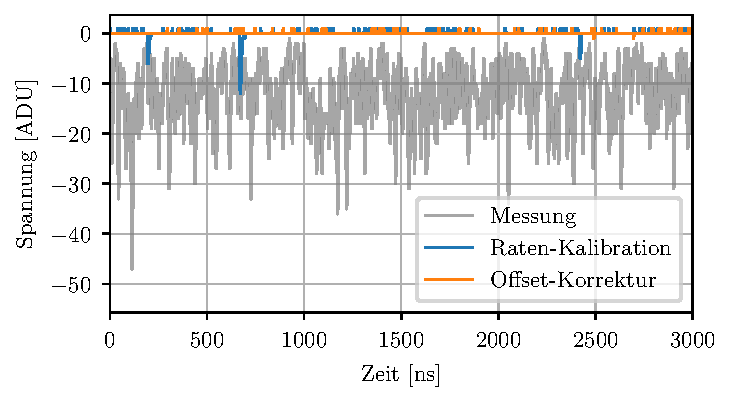
\includegraphics{images/Datenaufnahme/Kalibration.pdf}
    \caption{Abgebildet ist der Ausschnitt einer Waveform für die Offset Kalibration (ausgeschaltete Hochspannung und Beleuchtung), Raten-Kalibration (Hochspannung und Licht an, niedrige Photonenrate) und für die Messung.}
    \label{fig:Offest_Rate Kalibration}
\end{figure}

\subsection{Korrelation}
\label{ssec:Korrelation}
Die Korrelation der Daten erfolgt parallelisiert, nachdem die Datenaufnahme abgeschlossen ist. 
Jede Datei von beiden Kanälen wird getrennt miteinander korreliert, indem diese zuerst in Vektoren $\mathbf{A}$ und $\mathbf{B}$ eingelesen werden. 
Anschließend wird für jede Zeitdifferenz $\tau$ das folgende Skalarprodukt berechnet: 
\begin{equation}
    G^{(2)}(\tau) = \mathbf{A}(t)\cdot\mathbf{B}(t+\tau)
    \label{eq:korrelation}
\end{equation}
Damit entspricht jeder Wert von $G^{(2)}(\tau)$ der unnormierten zeitlichen Photonenkorrelation zu diesem Zeitpunkt \cite{zmijaOpticalIntensityInterferometry2021}. 
Die korrelierten Einzeldateien können anschließend für die weitere Datenanalyse gespeichert werden, da diese deutlich kleiner (im Bereich weniger kB) sind als die Rohdaten. 
Um aus einer bestimmten $G^{(2)}$-Funktion die normierte zeitliche Korrelationsfunktion zu erhalten, wird diese durch ihren Mittelwert weit außerhalb des Bunching Peaks geteilt:
\begin{equation}
    g^{(2)}(\tau) = \frac{G^{(2)}(\tau)}{\overline{G^{(2)}(\tau\gg\tau_c)}}
    \label{eq:G2 normalisierung}
\end{equation}
Ein Beispiel für die unnormierte Funktion $G^{(2)}$ einer einzelnen Datei ist in \autoref{fig:G2(tau)} dargestellt. 
\begin{figure}[h]
    \centering
    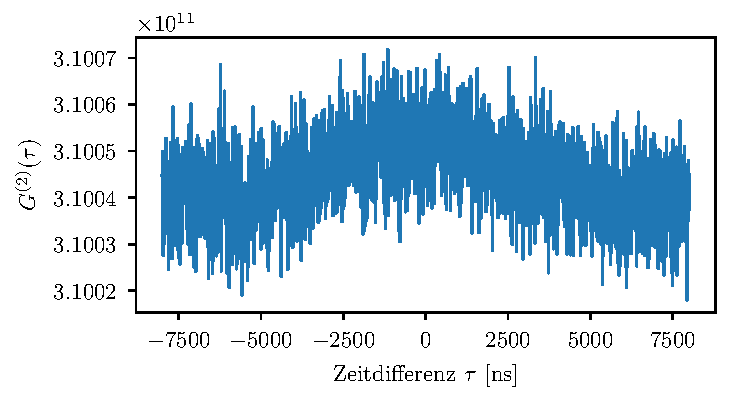
\includegraphics{images/Datenaufnahme/G2.pdf}
    \caption{Ein Beispiel einer unnormierten Korrelationsfunktion ist abgebildet. Durch das verrauschte Signal ist an der Stelle $\tau=0$ kein Bunching Peak sichtbar.}
    \label{fig:G2(tau)}
\end{figure}
Es ist ersichtlich, dass die Funktion stark verrauscht ist und der Bunching Peak nicht auszumachen ist. 
Die in \autoref{ssec:Intensitäteninterferometrie} bereits erwähnte Nowendigkeit der Mittelung über viele Daten, d. h. lange Zeiten, um die Form von $g^{(2)}$ bestimmen zu können, ist daher deutlich sichtbar. 

\subsection{Mittelung der Daten und Filter}
\label{ssec:mittelung und filter}
Wie bereits im vorangegangenen Abschnitt ersichtlich wurde, ist eine Mittelung vieler Dateien unumgänglich, um den Bunching Peak analysieren zu können. 
Hierbei wird der Ansatz eines gewichteten Mittelwerts gewählt, da nicht jede der etwa $3{,}4\,\mathrm{s}$ langen Dateien statistisch gleich aussagekräftig ist. 
So weisen manche der Messabschnitte höhere Photonenraten auf als andere (vgl. dazu \autoref{fig:Screenshot GUI}, Kasten \emph{5}). 
Unter der Annahme, dass ein Großteil des Rauschens in der $G^{(2)}$-Funktion statistischen Fluktuationen entspricht, wird erwartet, dass das Rauschen für höhere Photonenraten abnimmt. 
Dies bedeutet, dass Dateien mit höheren Raten und geringerer Schwankung stärker gewichtet werden sollten, als jede mit geringeren Photonenraten. 
Um dies zu bewerkstelligen, wird von jeder Datei $G^{(2)}_i$ die Standardabweichung $\sigma_i$ bestimmt und anschließend der folgende gewichtete Mittelwert berechnet \cite{cochranProblemsArisingAnalysis1937}:
\begin{equation}
    \overline{G^{(2)}} = \frac{\sum_{i=0}^{n}\frac{G^{(2)}_i}{\sigma_i^2}}{\sum_{i=0}^{n} \sigma_i^{-2}}
\end{equation}
Das Ergebnis der Mittelung über 10000 Dateien, d. h. etwa $9{,}5$\,h Korrelationsdaten, ist in \autoref{fig:gemittelte G2 vs g2} oben abgebildet. 
Der Bunching Peak bei $\tau\approx 0$ ist nach Mittelung der Daten bereits sichtbar. 
Allerdings sind durch die Mittelung weitere Artefakte ersichtlich geworden. 
Bereits in den korrelierten Einzeldateien ist eine Struktur in den Daten zu erkennen, welche das Signal überlagert. 
Nach der Mittelung ist diese nun besonders deutlich, was darauf hinweist, dass sie nicht von rein statistischer Natur ist, sondern tatsächlich zwischen den Kanälen korreliert ist. 
Das etwa $12\,\mathrm{\mu s}$ breite Störsignal kommt von der Spannungsversorgung der Xenonlampe \cite{zmijaOpticalIntensityInterferometry2021}, liegt daher in beiden Kanälen zugleich vor und wird deshalb durch die Korrelation und Mittelung verstärkt. 
Da es aber mehrere Größenordnungen breiter ist als der Bunching Peak und diesen daher kaum beeinflusst, wird es in diesem Abschnitt erst einmal vernachlässigt. 
In einem späteren Abschnitt zur Integration des Peaks wird auf eine Methode eingegangen, dieses Störsignal zu entfernen. \\
\begin{figure}[h]
    \centering
    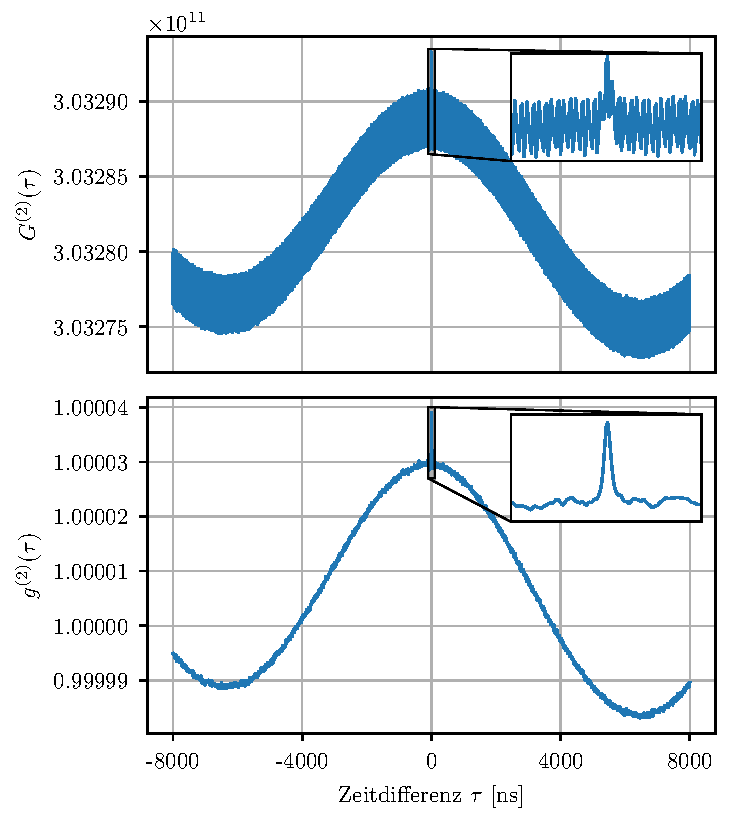
\includegraphics{images/Datenaufnahme/G2_vs_g2.pdf}
    \caption{Dargestellt sind der Unterschied zwischen $G^{(2)}(\tau)$ und der normierten Funktion $g^{(2)}(\tau)$ nach Mittelung über 10000 Dateien, bei der zudem die \glqq pattern correction\grqq\;und der Tiefpass angewandt worden sind. Es ist deutlich erkennbar, dass die angewandten Methoden zu einer starken Verbesserung des Signal-Rausch-Verhältnisses geführt haben. }
    \label{fig:gemittelte G2 vs g2}
\end{figure}

Weiterhin ist durch Zoom in die Daten oder eine Fouriertransformation dieser ein 8-Bin-periodisches Muster zu erkennen, welches dafür verantwortlich ist, dass die $G^{(2)}$-Funktion ein breites Band an Werten annimmt. 
Dieses von den ADC-Karten kommende Muster stört den Verlauf des Bunching Peaks zudem in beträchtlicher Weise, da es sich auf der selben Zeitskala wie der Peak selbst befindet. 
Da das Störsignal von den beiden ADC-Karten gleichzeitig ausgeht, ist dieses korreliert und daher besonders dominant in der abgebildeten $G^{(2)}$-Funktion.
Um das Störsignal zu entfernen, wird eine von der Arbeitsgruppe geschriebene \glqq pattern correction\grqq\;angewandt, welche in den ersten 4000 Bins (d. h. im Intervall $\tau\in[-8000,-1600]\,\mathrm{ns}$) jeweils 8 Bins mittelt und die Daten anschließend durch das so ermittelte Muster teilt. 
Da das Muster sowohl das eigentliche 8-Bin-periodische Muster, als auch den Offset der $G^{(2)}$-Funktion, wie er in \autoref{eq:G2 normalisierung} definiert ist, enthält, wird diese durch die Division automatisch auch normiert. 
Der Schritt der \glqq pattern correction\grqq\;wird für jede Datei separat vor der Bildung des Mittelwertes angewandt. \\
Nach diesen Schritten wird auf die gemittelte $g^{(2)}$-Funktion noch ein digitaler Tiefpass 2. Ordnung mit einer Grenzfrequenz von 200\,MHz angewandt, um weitere hochfrequente Störsignale zu entfernen. 
Die nach erwähnten Korrekturen und der angewandten Mittelung erhaltene Funktion $g^{(2)}(\tau)$ ist in \autoref{fig:gemittelte G2 vs g2} unten abgebildet. 


\clearpage
\mbox{}
\clearpage

\section{Analyse der Daten}
\label{sec:Analyse}
Im folgenden Abschnitt soll die Analyse der aufgenommenen Daten erfolgen. 
Dafür wird zuerst darauf eingegangen, wie der störende Untergrund in den Messdaten, der durch die Spannungsversorgung der Xenonlampe hervorgerufen wird, beseitigt werden kann. 
Anschließend wird auf die Integration des Bunching Peaks eingegangen, indem zuerst über die Konstruktion einer Theoriefunktion und deren Fit und anschließend über die Integration von dieser gesprochen wird. 
In diesem Zuge wird zudem kurz auf die Frage eingegangen, ob eine Integration der $g^{(2)}$-Funktion direkt oder eines Fits für die weitere Analyse sinnvoller ist. 
Danach wird erklärt, wie der Fehler auf die berechneten Integrale abgeschätzt wird. 
Nach diesen Schritten werden die ermittelten $\tau_c$ mit der theoretischen Erwartung aus \autoref{eq:tau_c_th} verglichen und diskutiert, ob ein Einfluss der Kabellänge auf $\tau_c$ vorliegt. 
Abschließend werden die erzielten Ergebnisse auf die Daten der H.E.S.S. Kampagne von 2022 angewandt. 

\subsection{Beiseitigung des niederfrequenten Störsignals in \texorpdfstring{$g^{(2)}(\tau)$}{g2}}
\label{ssec:Beseitigung des niederfrequenten Störsignals}
Wie in \autoref{ssec:mittelung und filter} angesprochen, ist das Signal, welches den Bunching Peak beinhaltet, überlagert von einem niederfrequenten Störsignal, welches von der Lampe hervorgerufen wird. 
Bevor das Integral des Peaks berechnet werden kann, muss dieses Störsignal entfernt werden. 
Betrachtet man Messreihen mit verschiedenen Kabellängen, fällt auf, dass das Störsignal nicht exakt identisch ist. 
Stattdessen ist dieses immer leicht unterschiedlich. 
Für die Entfernung muss also das Störsignal aus jeder Messreihe separat bestimmt und entfernt werden. 
Eine Möglichkeit hierfür wäre, einen Fit einer periodischen Funktion, z. B. $f(\tau) = a\cdot\mathrm{sin}(b(\tau-c))+d$ durchzuführen. 
Dies ist allerdings mit einigen Nachteilen verbunden. 
Betrachtet man das Störsignal (Abgebildet z. B. in \autoref{fig:gemittelte G2 vs g2}) genauer, fällt auf, dass dieses nicht symmetrisch ist. 
Um es voll zu erfassen, müsste $f(x)$ also noch um weitere Parameter ergänzt werden, was den Fit verkompliziert. 
Zusätzlich ist die Wahl der Fitfunktion letztlich arbiträr, da beliebige Parameter hinzugefügt werden können und keine Erwartung an die theoretische Form des Störsignals vorliegt. \\
Da der Bunching Peak und das Störsignal aber um Größenordnungen verschiedene zeitliche Ausdehnungen haben (ersterer grob 100\,ns, letzteres etwa 10{.}000\,ns), bietet es sich an, das Muster des Störsignals im Frequenzraum zu extrahieren. 
Dafür wird ein Tiefpassfilter zweiter Ordnung verwendet, dessen Grenzfrequenz so gewählt wird, dass lediglich die niederfrequenten Anteile des Signals extrahiert werden. 
Das ermittelte Muster kann anschließend von $g^{(2)}(\tau)$ abgezogen werden, was den Offset entfernt und dafür sorgt, dass außerhalb des Bunching Peaks etwa $g^{(2)}\approx 0$ gilt. 
Für die Wahl der richtigen Grenzfrequenz ist es nützlich, \autoref{fig:lf_offset für verschiedene Grenzfrequenz} zu betrachten
In dieser ist abgebildet, wie das ermittelte Muster für verschiedene Grenzfrequenzen aussieht. 
\begin{figure}[h]
    \centering
    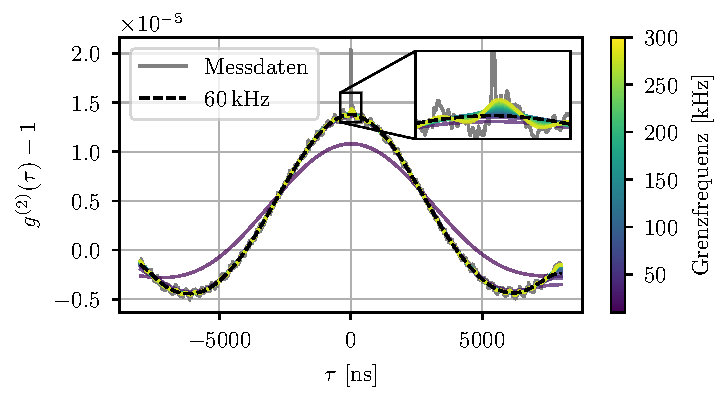
\includegraphics{images/Analysis/lf_offset.pdf}
    \caption{Gezeigt ist ein Vergleich der extrahierten Muster für verschiedene Grenzfrequenzen. In Grau ist die gemittelte $g^{(2)}$-Funktion, aufgenommen mit der Kabelkombination Airborne 5 $40\times 40$ Meter, dargestellt. Farbig hinterlegt sind die ermittelten Muster für verschiedene Grenzfrequenzen. Es ist offensichtlich, dass bei niedrigen Grenzfrequenzen Muster entstehen, die das Störsignal nicht voll erfassen (lila), und bei hohen Grenzfrequenzen (gelb) Muster entstehen, welche Amplitude vom Bunching Peak abschneiden. Eine gute Grenzfrequenz, die das Störsignal großflächig abdeckt und gleichzeitig keine feine Struktur erfasst, liegt bei 60\,kHz und ist schwarz gestrichelt eingezeichnet.}
    \label{fig:lf_offset für verschiedene Grenzfrequenz}
\end{figure}
In der Abbildung ist ersichtlich, dass sowohl zu niedrige als auch zu hoch gewählte Grenzfrequenzen problematisch sind. 
Zu niedrig gewählte Grenzfrequenzen sorgen dafür, dass das Störsignal nicht vollständig erfasst wird (vgl. lila Kurve in \autoref{fig:lf_offset für verschiedene Grenzfrequenz}). 
Je niedriger die Frequenz wird, desto mehr wird statt des gesamten Signals nur dessen Mittelwert extrahiert. 
Eine Subtraktion dieses Musters würde dann dazu führen, dass das Störsignal noch immer vorliegt und lediglich eine geringere Amplitude aufweist. 
Wählt man allerdings die Grenzfrequenz zu hoch, so werden Teile des höherfrequenten Signals der $g^{(2)}$-Funktion fälschlicherweise als Störsignal erkannt. 
Im Extremfall wird so ein Teil des Bunching Peaks bei der Subtraktion abgezogen, was das Ergebnis für $\tau_c$ verfälschen würde. 
Dies ist in \autoref{fig:lf_offset für verschiedene Grenzfrequenz} gelb eingezeichnet. \\
Es gilt also eine Grenzfrequenz zu finden, welche das Störsignal zwar großflächig vollständig erfasst, aber möglichst keinen Einfluss auf die Feinstruktur der Korrelationsfunktion hat. 
Diese Frequenz wird zu etwa 60\,kHz bestimmt. 
Zur Veranschaulichung ist das mit einer Grenzfrequenz von 60\,kHz ermittelte Muster schwarz gestrichelt in \autoref{fig:lf_offset für verschiedene Grenzfrequenz} eingezeichnet. \\

Nach dem Berechnen des Musters wird dieses von der $g^{(2)}$-Funktion abgezogen. 
Durch dieses Vorgehen, erhält man die Korrelationsfunktion, welche in \autoref{fig:g2-offset} dargestellt ist.
\begin{figure}[h]
    \centering
    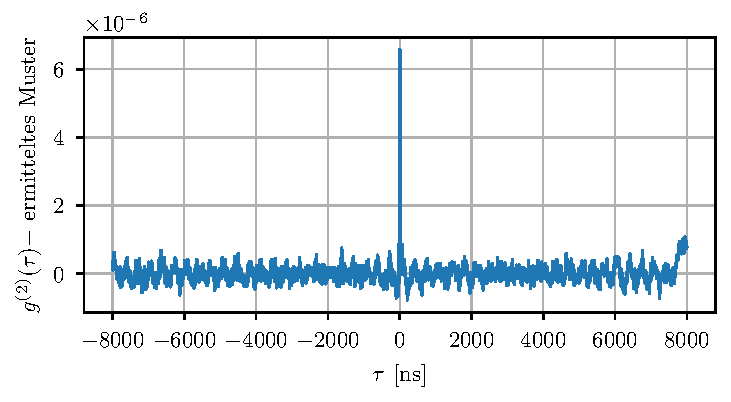
\includegraphics{images/Analysis/g2-lf_offset.pdf}
    \caption{Hier ist dargestellt, wie die $g^{(2)}$-Funktion nach Subtraktion des ermittleten niederfrequenten Störmusters aussieht. Der Bunching Peak sticht nun sehr klar aus dem Hintergrund heraus, welcher um den Wert 0 schwankt.}
    \label{fig:g2-offset}
\end{figure}
Es ist ersichtlich, dass die beschriebene Methode den niederfrequenten Offset im Signal gut entfernt. 
Ein weiterer Vorteil dieser Methode ist, dass der Hintergrund nun um den Wert 0 schwankt, sodass ein Offset in y-Richtung für die spätere Integration (und den Fit) nicht berücksichtigt werden muss. \\
Allerdings soll hier auch auf die Limitationen des erwähnten Vorgehens hingewiesen werden. 
Erstens ist auffällig, dass $g^{(2)}(\tau)$ für $|\tau|\gtrsim 6000\,\mathrm{ns}$ von der Schwankung um 0 abweicht und stattdessen wieder größer wird. 
Dies liegt daran, dass der Tiefpass diese Randregionen aufgrund des abgeschnittenen Signals nicht mehr gut erfassen kann. 
Tatsächlich ist auch schon in \autoref{fig:lf_offset für verschiedene Grenzfrequenz} ersichtlich, dass das extrahierte Muster in den Randregionen stets zu niedrig ist und daher nach der Subtraktion zu hohe Werte liefert. 
Da der Bunching Peak aber für alle verwendeten Kabelkombinationen bei $\tau\approx 0$ liegt, ist die Auswirkung dieser Randbereiche auf $\tau_c$ vernachlässigbar. 
Trotzdem wird für alle folgenden Analyseabschnitte der Definitionsberiech der Offset-korrigierten $g^{(2)}$-Funktion auf $\tau\in[-6000,6000]\,\mathrm{ns}$ eingeschränkt, um einen Einfluss dieser Randeffekte (besonders auf den Fehler auf $\tau_c$, vgl. \autoref{ssec:Fehler von tau_c}) vermeiden zu können. 
Von größerem Belang ist allerdings die Wahl der Grenzfrequenz selbst. 
Wie oben beschrieben erfolgte diese hier anhand von visuellen Überlegungen anhand der $g^{(2)}$-Funktion und dem ermittelten Muster. 
Da sich aber für verschiedene Grenzfrequenzen leicht andere Werte des Musters bei $\tau\approx 0$ ergeben, wirken sich diese auch auf das Integral aus. 
Durch das Festlegen der Grenzfrequenz per Auge ergibt sich ein relativ großer Wertebereich an möglichen Grenzfrequenzen, welche alle ähnlich plausibel erscheinen. 
Die hier gewählten 60\,kHz stellen so etwa die Mitte eines $\pm20\,\mathrm{kHz}$ breiten Bereichs dar. 
Der geschätzte systematische Fehler auf das Integral anhand der später entwickelten Integrationsstrategie liegt im niedrigen einstelligen Bereich. \\

Da dies, wie später klar wird, in der Größenordnung des statistischen Fehlers auf $\tau_c$ liegt, soll an dieser Stelle bereits auf die Notwendigkeit verwiesen werden, für weitere Labormessungen eine tiefergehende Untersuchung bezüglich der Wahl der Grenzfrequenz anzustellen. 
Diese sollte zum Ziel haben, eine besser gerechtfertigte Wahl für die Grenzfrequenz treffen zu können und den systematischen Fehler, der durch die Festlegung dieser Frequenz entsteht, besser zu quantifizieren. 
Da diese Untersuchungen allerdings den Rahmen dieser Arbeit überschreiten würden, wird im Folgenden von einer festen Grenzfrequenz von 60\,kHz ausgegangen, welche, wie in \autoref{fig:g2-offset} zu sehen, bereits zu guten Ergebnissen führt. 

\subsection{Fitfunktion}
\label{ssec:Fitfunktion}    
Nachdem der Offset der Korrelationsfunktion nun abgezogen ist, kann an das Integrieren dieser gedacht werden. 
Dafür sollen in einem späteren Abschnitt verschiedene Integrationsmethoden und Integrationsbereiche miteinander verglichen werden, darunter auch die Integration eines Fits. 
Für diesen späteren Abschnitt ist es also nötig, eine Funktion zu finden, welche den Bunching Peak treffend beschreibt. 
Dies soll das Ziel des jetzigen Abschnittes sein. 

\subsubsection{Bisherige Herangehensweise: Korrelierte gemittelte PMT-Pulse und Gaußfunktion}
\label{sssec:Fitfunktion - Bisherige Herangehensweise}
In der Arbeitsgruppe existieren verschiedene Ideen darüber, welche Fitfunktionen geeingnet sind. 
So wurden für die ersten Labormessungen z. B. gemessene gemittelte Photonenpulse, die während der Ratenkalibration aufgenommen werden (vgl. \autoref{ssec:Datenaufnahme und Waveforms}), korreliert, linear interpoliert und an die Daten gefittet \cite{zmijaOpticalIntensityInterferometry2021}. 
Dies ergibt Sinn, da sich die Ausgangspulse der PMTs (wie in \autoref{ssec:Datenaufnahme und Waveforms} beschrieben) über einige Bins erstrecken und so das zeitlich sehr schmale Bunching Signal verwaschen. 
Die Erwartung an den Bunching Peak in den korrelierten Daten ist daher, dass er sich wie die PMT-Pulse über einige Bins erstreckt und etwa der Form der korrelierten mittleren Pulsform entspricht. \\
Eine weitere Herangehensweise liegt im Fit einer Gaußfunktion an das Signal. 
Dies entspricht der momentanen Herangehensweise der Arbeitsgruppe und wurde z. B. für die Auswertung der Daten der H.E.S.S. Kampagne von 2022 verwendet \cite{zmijaFirstIntensityInterferometry2023}. 
Vorteil dieser Methode ist die relativ einfache, analytische Funktion, welche an die Daten gefittet wird. 
Während bei der vorherigen Methode Daten korreliert und dann interpoliert werden müssen, um die Interpolationsfunktion daraufhin numerisch zu integrieren, kann für die Integration einer Gaußfunktion auf eine simple Formel zurückgegriffen werden:
\todo{cite}
\begin{equation}
    \tau_c^{\mathrm{meas}} = \sqrt{2\pi} a\sigma
\end{equation}
Hierbei sind $a$ die Amplitude und $\sigma$ die Breite der gefitteten Gaußfunktion. 
Dieses Vorgehen vereinfacht den Fit und erlaubt es, relativ einfach Fitparameter wie den Mittlelwert und die Breite $\sigma$ festzuhalten, was aufgrund niedriger Statistik z. B. für die Daten von 2022 nötig war \cite{zmijaFirstIntensityInterferometry2023}. 
Allerdings hat diese Methode auch einen Nachteil, welcher in \autoref{fig:g2-fit Gauß} visualisiert ist. 
\begin{figure}[h]
    \centering
    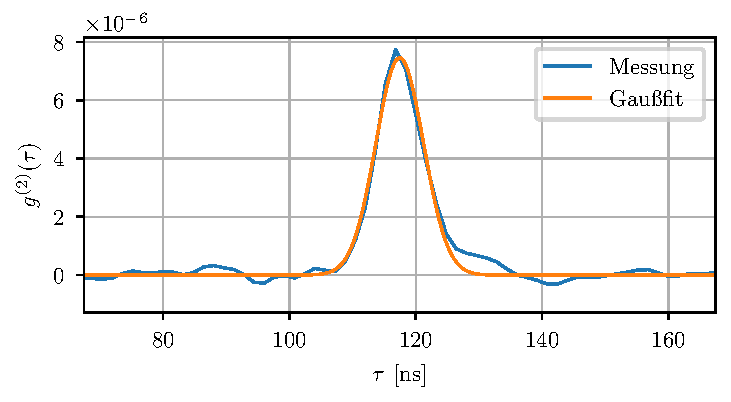
\includegraphics{images/Analysis/g2_gaussfit.pdf}
    \caption{Gezeigt sind die $g^{(2)}$-Funktion für die Messung mit 10\,m und 40\,m Kabeln des Typs Airborne 5. Zusätzlich ist der Fit einer Gaußfunktion eingezeichnet.}
    \label{fig:g2-fit Gauß}
\end{figure}
Durch die Verwendung verschiedener Kabellängen und damit unterschiedlicher Dispersion des Signals für jeden Kanal, folgt für den Bunching Peak als Korrelation der beiden Kanäle, dass dieser asymmetrisch ist. 
Diese Asymmetrie kann vom Gaußfit nicht vollständig erfasst werden -- es wird lediglich die mittlere Abweichung des Fits zu den Datenpunkten minimiert. 
Wie in \autoref{fig:g2-fit Gauß} ersichtlich, werden besonders die Randbereiche des Peaks nicht vom Gaußfit erfasst. 
Da benachbarte Bins allerdings Korrelationen aufweisen und der Bunching Peak über mehrere Bins ausgedehnt ist, enthalten auch die Randbereiche des Peaks das Signal korrelierter Photonen. 
In der vorliegenden Arbeit soll daher, gerade weil es die höhere Statistik der Labormessungen zulässt, von ersterer Methode ausgegangen werden. 
Die Schritte bis zur fertigen Fitfunktion werden im Folgenden erläutert.

\subsubsection{Neue Herangehensweise: Faltung beider Funktionen}
\label{sssec:Fitfunktion - Meine Herangehensweise}
Wie bereits angesprochen verändert sich die Form der Pulse, abhängig von der Kabellänge, die diese durchlaufen. 
In \autoref{fig:mittlere Pulsform} sind zur Veranschaulichung zwei mittlere PMT-Pulse nach Durchlauf eines 40 bzw. 10\,m langen Airborne 5 Kabels dargestellt. 
Diese werden, wie in \autoref{ssec:Datenaufnahme und Waveforms} erwähnt, von der Aufnahmesoftware automatisch gespeichert. 
\begin{figure}[h]
    \centering
    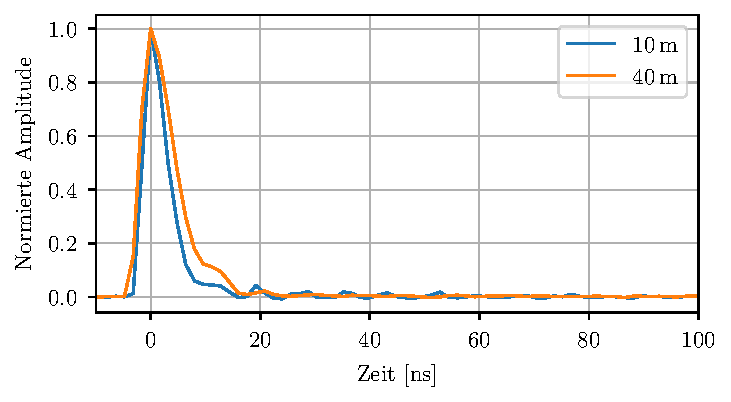
\includegraphics{images/Analysis/mean_pulseshapes.pdf}
    \caption{Gezeigt sind Ausschnitte der mittleren Pulsform bei Verwendung eines 40\,m bzw. 10\,m Airborne 5 Kabels. Es ist erkennbar, dass der orangene Puls breiter als der blaue ist, was an der erhöhten Dispersion im längeren Kabel liegt. Weiterhin wird eine stärkere Dämpfung, d. h. eine Abnahme der Amplitude für längere Kabel, erwartet, was hier aber aufgrund der Normierung nicht direkt sichtbar ist.}
    \label{fig:mittlere Pulsform}
\end{figure}
Wie erwartet, ist der Puls durch das längere Kabel sichtbar verbreitert. 
Im Anschluss werden die beiden mittleren Pulse miteinander korreliert (vgl. \autoref{eq:korrelation}), wobei darauf geachtet wird, dass bei kombinierten Daten von mehreren Messungen auch die aufgenommenen Pulse vor der Korrelation gemittelt werden. 
Zur besseren Interpretation der Parameter in der späteren Funktion wird der so erhaltene Vektor an Datenpunkten zusätzlich normiert, indem durch sein Maximum geteilt wird und so in der Zeit verschoben, dass das Maximum bei $\tau=0$ liegt. 
Da bisher noch keine Funktion, sondern lediglich Datenpunkte vorliegen, wird anschließend eine lineare Interpolation durchgeführt, um die Funktion $y(\tau)$ zu erhalten. 
Diese ist zusammen mit den Datenpunkten der korrelierten Pulsform in \autoref{fig:Interpolation} gezeigt. 
\begin{figure}[h]
    \centering
    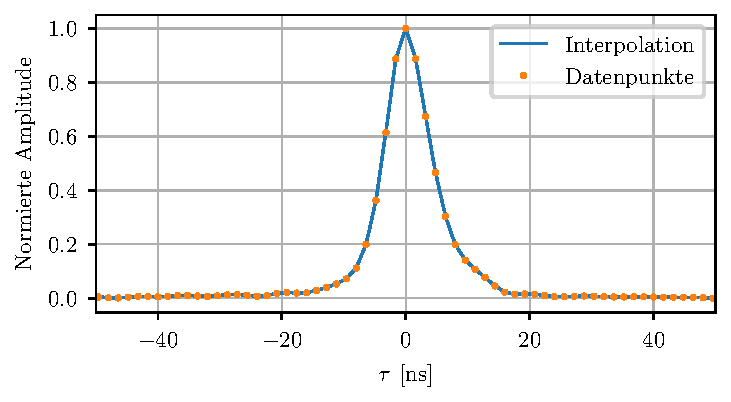
\includegraphics{images/Analysis/interpolation.pdf}
    \caption{Dargestellt ist das Ergebnis der diskreten Korrelation (orange) und die lineare Interpolation davon (blau).}
    \label{fig:Interpolation}
\end{figure}
Die so ermittelte Funktion $y(\tau)$ kann nun durch freie Parameter ergänzt werden, sodass diese an die Datenpunkte der $g^{(2)}$-Funktion gefittet werden kann. 
Notwendig sind ein Offset in x-Richtung $\tau_0$ und ein Amplitudenfaktor $a$, welcher den Fit in y-Richtung staucht und streckt. 
Weiterhin kann eine Streckung des Peaks in x-Richtung im Vergleich zu $y(\tau)$ vorliegen, was auf eine Veränderung in der Zeitauflösung der Messung im Vergleich zur Kalibration zurückzuführen ist. 
Da für die Konstruktion der korrelierten mittleren Photonenpulse Photonenpeaks der Raten-Kalibrationsmessung zuerst übereinander verschoben und anschließend gemittelt werden, enthält $y$ bereits die Zeitauflösung des Systems, welches durch das Binning bedingt ist. 
Eine zusätzliche Verbreiterung des Bunching Peaks im Vergleich zu $y(\tau)$ wäre daher auf eine zusätzliche statistische Schwankung der Position des Bunching Peaks zurückzuführen, welche in der Kalibrationsmessung nicht vorliegt. 
Beispiele hierfür sind zeitliche Schwankungen der PMT-Ausgangssignale oder eine durch das Teleskop selbst bedingte Verschlechterung der Zeitauflösung (vgl. \autoref{ssec:Vergleich mit Hess}).

Um diesen möglichen Effekt in der Fitfunktion zu quantifizieren, wird eine Vorgehensweise ähnlich der in \cite{lasseguesFieldIntensityCorrelations2022} gewählt, bei der die Funktion $y(\tau)$, welche der Theoriefunktion bei idealer Zeitauflösung entspricht, mit einer Gaußfunktion gefalten, welche über ihre Breite $\sigma$ eine zusätzliche Verschlechterung der Zeitauflösung ausdrückt. 
Es folgt:
\begin{equation}
    f(\tau, a, \sigma, \tau_0) = ay(\tau - \tau_0) * \mathrm{e}^{-\frac{\tau^2}{2\sigma^2}}
\end{equation}
Weil die verwendete Routine zur Faltung nur für Vektoren und nicht für Funktionen definiert ist, ergeben sich in der Auswertung noch leichte Abweichungen von dieser Vorgehensweise. 
So werden die linke und rechte Seite der Faltung erst in einem ausreichend großen und fein gewählten Intervall unter Einsetzung der Parameter $a=1$ und $\tau_0 = 0$ ausgewertet, woraufhin die diskrete Faltung der beiden Vektoren durchgeführt wird. 
Um anschließend wieder eine Funktion zu erhalten, welche für alle $\tau$ definiert ist, wird erneut eine lineare Interpolation durchgeführt und normiert, was zu Funktion $h$ führt. 
Schlussendlich ergibt sich die Fitfunktion also zu:
\begin{equation}
    f(\tau, a, \tau_0, \sigma) = ah(\tau- \tau_0, \sigma)
    \label{eq:fit funktion final}
\end{equation} 
Durch die Variation der Parameter während der Fitroutine geht der Parameter $\sigma$ dann vor der Faltung ein, während die $a$ und $\tau_0$ nach der Faltung und Interpolation eingehen. 
Durch die erwähnten Normierungs- und Verschiebungsschritte der Funktionen, welche die Funktion $f$ bilden, entspricht (bis auf für den Fit unwesentliche Abweichungen) $a$ nun der Amplitude des Fits und $\tau_0$ seinem Offset von $\tau=0$. 
Auf diese Weise ist eine Einschränkung der Fitparameter für die spätere Auswertung möglich, was die Konvergenz der Fits verbessert. 
Die Größe von $\sigma$ beschreibt eine mögliche systembedingte Zeitauflösung während der Messung, welche während der Kalibration nicht vorliegt. 
Wie eine Variation des Fitparameters $\sigma$ die resultierende Funktion $f$ beeinflusst, ist in \autoref{fig:Fitfuktion für verschiedene sigma} für $a=1$, $\tau_0=0$ dargestellt. 
\begin{figure}[h]
    \centering
    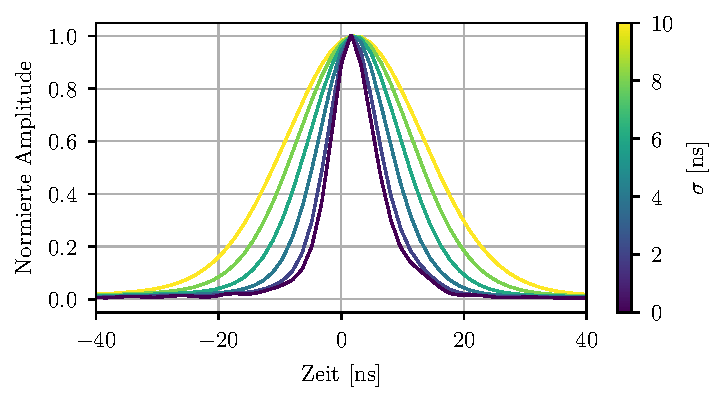
\includegraphics{images/Analysis/corr_pulses_diff_sigma.pdf}
    \caption{Dargestellt ist ein Ausschnitt der resultierenden Fitfunktion $f$ bei Variation des Fitparamters $\sigma$ ($a=1$, $\tau_0=0$). Für sehr niedrige $\sigma$ entspricht die Funktion praktisch der korrelierten Pulsform der PMTs und für größer werdende $\sigma$ nähert sich die Funktion immer mehr der Form einer Gaußfunktion an.}
    \label{fig:Fitfuktion für verschiedene sigma}
\end{figure}
Es ist ersichtlich, dass eine Erhöhung des Parameters $\sigma$ zu einer Verbreiterung der Fitfunktion führt, welche zudem immer glatter und gaußförmiger wird. \\

Die Konstruktion und Verwendung der Fitfunktion, wie oben beschrieben, hat einige Vorteile. 
Wie bereits angesprochen, entspricht eine Faltung von einer Gaußfunktion, welche die Zeitauflösung während der Messung enthält, mit der gemessenen erwarteten Peakform bei bestmöglicher Zeitauflösung am ehesten der theoretischen Erwartung an die Form des Bunching Peaks. 
Zudem werden durch dieses Vorgehen eine mögliche Asymmetrie des Peaks und Ringing der PMTs berücksichtigt, was zu einer genaueren Bestimmung des Integrals und damit der Kohärenzzeit führt. 
Durch die Veränderung der korrelierten Pulsform für jede Kabellängenkombination ändert sich auch die Fitfunktion und bildet so die kabelabhängige Form des Bunching Peaks besser ab. 
Zusätzlich kann durch dieses Vorgehen die Zeitauflösung des Systems aus den gemessenen Daten bestimmt werden. 
Aus diesen Gründen wird im Folgenden auf die soeben beschriebene Fitfunktion zurückgegriffen. 

\subsection{Wahl der Integrationsmethode und Integrationsgrenzen}
\label{ssec:Wahl der Integrationsmethode}
Zur Vollständigkeit soll in diesem Analyseteil kurz darauf eingegangen werden, ob ein Fit an die Daten notwendig ist oder ob es ausreicht, die gemittelte $g^{(2)}$-Funktion direkt zu integrieren. 
Im selben Zuge wird die Wahl der Integrationsgrenzen für die spätere Analyse motiviert. 
Hierfür wird exemplarisch ein Fit von \autoref{eq:fit funktion final} an die gemittelten, Offset-korrigierten Daten der Airborne $10\times 10\,\mathrm{m}$-Messung durchgeführt. 
Anschließend werden sowohl der Fit als auch die Daten selbst numerisch integriert. 
Der Fit erfolgt in einem breiten Intervall von $\pm 100$ Bins, d. h. $\pm 160\,\mathrm{ns}$ um den Peak herum. 
Die Integration erfolgt in einem Intervall $[\tau_{\mathrm{max}}-w, \tau_{\mathrm{max}}+w]$, wobei $\tau_{\mathrm{max}}$ dem Zeitpunkt entspricht, an welchem $g^{(2)}(\tau)$ maximal ist und die Integrationsbreite $w$ im Bereich $w\in [1,160]\,\mathrm{ns}$ variiert wird. 
Das Resultat dieser Analyse ist in \autoref{fig:integration verschiedene Breiten} dargestellt. 
\begin{figure}[hp]
    \centering
    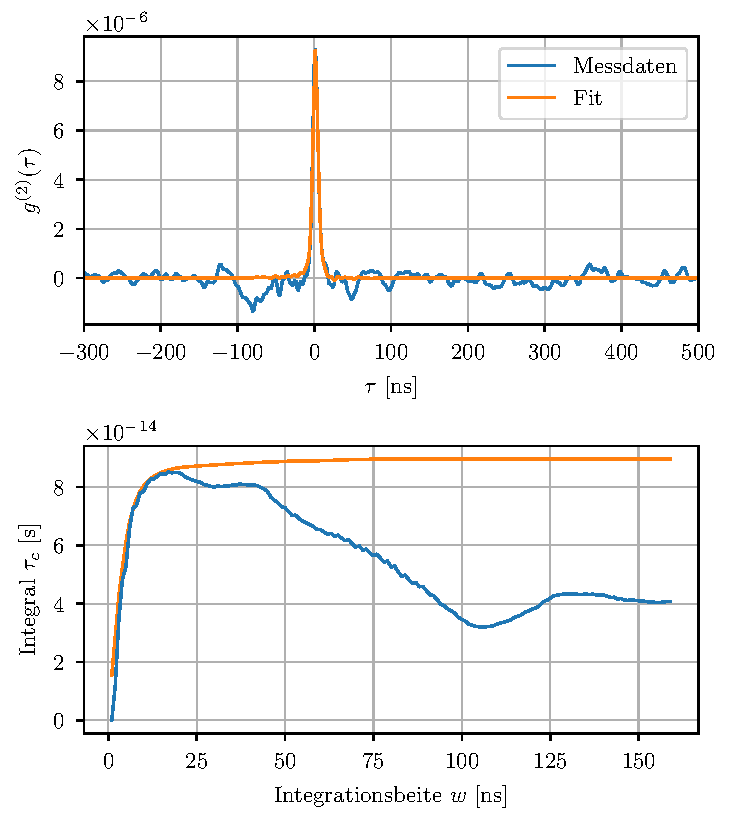
\includegraphics{images/Analysis/integration_different_width.pdf}
    \caption{Oben ist die $g^{(2)}$-Funktion (blau) sowie ein Fit an diese (orange) zu sehen. Für verschiedene Integrationsbreiten ist unten in gleichen Farben abgebildet, wie sich die resultierenden Integrale der beiden Funktionen entwickeln. Für die Integration der Rohdaten ist eine deutliche Fluktuation des Integrals zu sehen, während die Integration des Fits sich auch für große Breiten stabil verhält.}
    \label{fig:integration verschiedene Breiten}
\end{figure}
In der Grafik ist erkennbar, dass die Integration des Fits für steigende Integrationsbreiten zunimmt und schließlich einen stabilen Wert annimmt. 
Dies ergibt Sinn, da die Interpolation der Daten im letzten Schritt der Konstruktion der Fitfunktion außerhalb des Bereichs der Datenpunkte den konstanten Wert 0 annimmt. 
Da weiterhin kein y-Offset gefittet wird, ändert sich das Integral ab einer gewissen Integrationsbreite daher nicht mehr. 
Die direkte Integration der Messdaten hingegen ist stark abhängig von Fluktuationen der Korrelationsfunktion außerhalb des Bunching Peaks. 
So sinkt diese z. B. zwischen $w=50\,\mathrm{ns}$ und $w=100\,\mathrm{ns}$ stark, was an dem zufällig niedrigen Wert der Korrelationsfunktion links vom Bunching Peak (vgl. \autoref{fig:integration verschiedene Breiten} oben) liegt. \\

Da ein Ziel dieser Arbeit sein soll, Integrale verschiedener Kabellängen miteinander zu vergleichen und es keine von vornherein \glqq richtige\grqq\;Wahl der Integrationsbreite gibt, welche nur Signal und kein Rauschen erfasst, ist Stabilität im Wert von $\tau_c$ für verschiedene Integrationsbreiten essentiell. 
Da benachbarte Bins wie erwähnt korreliert sind, sind häufig breite Fluktuationen von $g^{(2)}(\tau)$ nach unten oder oben anzutreffen, welche die Differenz zwischen Integralen für eine beliebige Integrationsbreite stark beeinflusst. 
Aus dem Grund der besseren Vergleichbarkeit der Messreihen untereinander wird daher die Methode gewählt, einen Fit von \autoref{eq:fit funktion final} an die Daten durchzuführen und diesen anschließend zu integrieren. 
Aus erwähnter Konstruktion mittels Interpolation und aus \autoref{fig:integration verschiedene Breiten} unten wird weiterhin ersichtlich, dass sich das Integral lediglich bis $w\approx 100\,\mathrm{ns}$ nennenswert ändert. 
Als Integrationsbreite ist also ein Wert von $w\gtrsim 100\,\mathrm{ns}$ geeignet, wobei ein zu großer Intervall per Konstruktion wie erwähnt keine Probleme verursacht. 
Aus diesem Grund wird die Funktion $f(\tau, a, \tau_0, \sigma)$ für die folgende Analyse stets in einem Intervall von $\pm 100$ Bins bzw. $\pm 160\,\mathrm{ns}$ gefittet und integriert. 

\subsection{Fehler von \texorpdfstring{$\tau_c$}{tc}}
\label{ssec:Fehler von tau_c}
Nachdem im vorigen Abschnitt auf das Integrieren des Bunching Peaks eingegangen wurde, soll im Folgenden der Fehler ebendieses Integrals abgeschätzt werden. 
Durch die Korrelation benachbarter Bins lässt sich nicht ohne weiteres ein Fehler auf den Wert der Korrelationsfunktion bestimmen, welcher durch den Fit fortgepflanzt werden kann, da die verwendete $\chi^2$-Minimierung statistisch unabhängige Fehler zwischen Samples voraussetzt \cite{vugrinConfidenceRegionEstimation2007}. 
Stattdessen wird eine andere Methode genutzt, welche das Rauschen der $g^{(2)}$-Funktion unmittelbar mit einbezieht. 
Dafür wird zuerst wie im letzten Abschnitt beschrieben ein Fit an den Bunching Peak durchgeführt, welcher daraufhin integriert wird, um den Wert für $\tau_c$ zu erhalten. 
Um anschließend auf den Fehler zu schließen, wird ebendieser Fit in feinen Schritten über die $g^{(2)}$-Funktion verschoben und zu dieser an der jeweiligen Stelle addiert. 
Es wird der Fit an die Daten, statt der Bunching Peak selbst, verschoben, um lediglich das Signal, nicht aber das umliegende Rauschen mitzuverschieben, welches einen systematischen Einfluss auf den Verlauf des Rauschens um den verschobenen Peak hätte. 
Der so erhaltene Peak entspricht jenem, der gemessen worden wäre, wenn das Rauschen um den Peak zufällig anders verschoben wäre. 
Da der hauptsächliche Fehler auf das Integral der zufälligen Position des Peaks in der $g^{(2)}$-Baseline entspricht (im Besonderen, ob der Peak auf einer niedrigen oder hohen Fluktuation liegt), lässt sich durch die Änderung des Integrals bei verschiedener Peakposition der Fehler auf das Integral gut abschätzen. 
Für jede Peakposition wird anschließend erneut mit derselben Methodik gefittet und integriert. 
Das Resultat dieses Vorgehens ist eine Liste an Integralen. 
Für den Fehler auf das Integral wird abschließend die Standardabweichung dieser Liste bestimmt, um zu quantifizieren, wie stark die Integrale im Mittel unter dem Einfluss des Rauschens in der Baseline schwanken. 
Die Standardabweichung als Maß für den Fehler zu wählen, ergibt an dieser Stelle Sinn, da die Schwankung der Baseline als näherungsweise gaußverteilt angenommen werden kann. 
Dies liegt daran, dass die Wahrscheinlichkeitsverteilung der Intensitätsfluktuationen einer chaotischen Lichtquelle für $\tau\gg \tau_c$ der Poissonverteilung des kohärenten Lichts um $g^{(2)}=1$ entspricht, was für hohe Photonenzahlen in eine Gaußverteilung übergeht \cite[Kap. 5.5]{foxQuantumOpticsIntroduction2006}.
Obwohl diese Fluktuationen sich in der Theorie exakt kürzen (vgl. \autoref{eq:g2_final}), sodass $g^{(2)}(\tau \gg \tau_c) = 1$, ist dies im Experiment aufgrund der Unterteilung in Zeitbins, Messabschnitte und weiterer Effekte nicht der Fall, sodass eine gaußverteilte Schwankung um die 1 verbleibt. \todo{macht das sinn?} \\

Exemplarisch ist das oben erklärte Vorgehen für die $10\times 10\,\mathrm{m}$-Airborne 5 Messung in \autoref{fig:Fehler auf tc} gezeigt. 
\begin{figure}[hp]
    \centering
    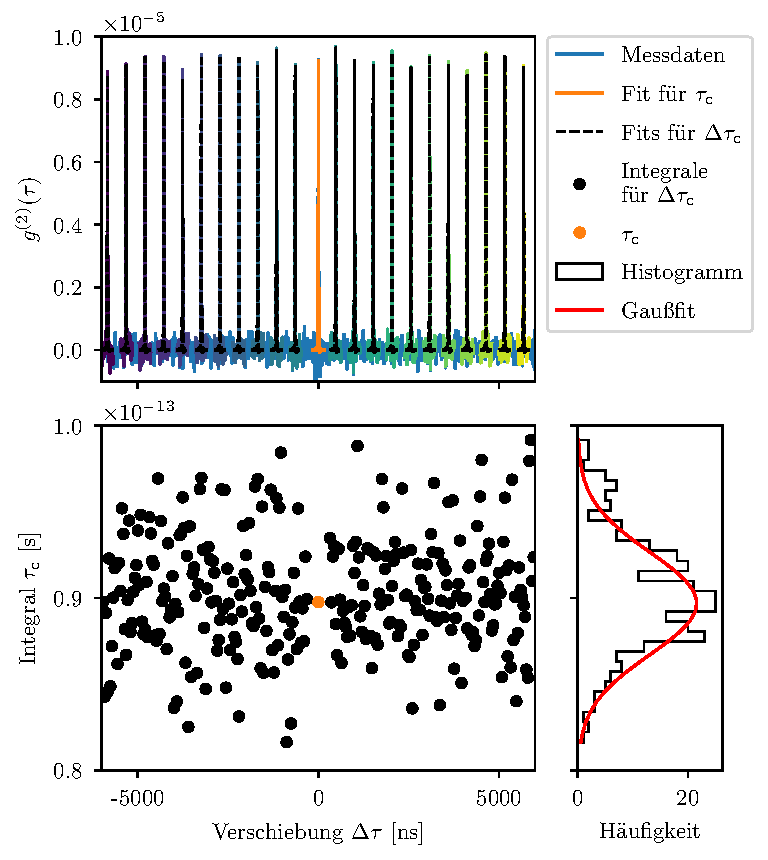
\includegraphics{images/Analysis/integration_error.pdf}
    \caption{Oben sind die gemittelte $g^{(2)}$-Funktion (blau), der Fit des Bunching Peaks (orange), die verschobenen und zur Baseline addierten Peaks (Farbgradient lila-gelb, je nach Verschiebung) und die erneut durchgeführten Fits an diese (schwarz gestrichelt) dargestellt. Unten links sind die reultierenden Integrale der verschobenen Fits und des Fits an den Bunching Peak (entspricht der Verschiebung $\Delta\tau=0$) im selben Farbschema dargestellt. Zur Bestimmung des Fehlers $\sigma_{\tau_c}$ wird die Standardabweichung der Verteilung der schwarzen Punkte berechnet, während $\tau_c$ dem orangenen Punkt entspricht. Unten rechts ist abschließend die Verteilung der schwarzen Punkte histogrammiert. Weiterhin ist ein Gaußfit (rot) durchgeführt worden, dessen Verlauf die Erwartung bestätigt, dass die Verteilung der Integrale gaußverteilt ist.}
    \label{fig:Fehler auf tc}
\end{figure}
Zuerst erfolgt im obigen Graph der Fit und die Integration des Bunching Peaks. 
Für alle Fits wurden erneut Fit- und Integrationsfenster von $\pm 100$ Bins gewählt (vgl. \autoref{ssec:Wahl der Integrationsmethode}). 
Anschließend wird die Fitfunktion in $25\,ns$-Schritten zwischen $\tau = -6000\,\mathrm{ns}$ und $\tau = 6000\,\mathrm{ns}$ verschoben, wobei darauf geachtet wird, die Region des ursprünglichen Bunching Peaks auszulassen. 
Der verschobene Peak wird auf die $g^{(2)}$-Baseline addiert, was im angesprochenen Graph als Farbverlauf (der Übersichtlichkeit wegen nur für wenige Verschiebungen) eingezeichnet ist. 
Für jede Verschiebung wird erneut ein Fit durchgeführt und integriert, was im unteren linken Teil der \autoref{fig:Fehler auf tc} als schwarzer Punkt aufgetragen ist. 
Wird nun die Standardabweichung der schwarzen Punkte (d. h. der Integrale für verschiedene Verschiebungen) gebildet, lässt sich damit wie oben beschrieben der Fehler auf $\tau_c$ bestimmen. 
Zur Verifikation der Annahme einer Gaußvertielung der Integrale, die in die Berechnung des Fehlers mit eingeht, ist unten links zudem ein Histogramm der angenommenen Integralwerte gegeben. 
An dieses wurde ein Fit einer Gaußfunktion durchgeführt, welche in guter Übereinstimmung mit der Verteilung der Punkte ist. 
Wie anhand theoretischer Überlegungen erwartet, ist eine Gaußverteilung also eine gerechtfertigte Annahme an die Verteilung der Änderung der Integrale mit verschiedenem $\Delta\tau$. 
Dies bestätigt, dass die gewählte Methode, insbesondere die Berechnung der Standardabweichung, geeignet ist, um die Schwankung der Integrale und daher $\sigma_{\tau_c}$ zu quantifizieren. 

\subsection{Ergebnisse für verschiedene Kabelkombinationen}
\label{ssec:Ergebnisse für verschiedene Kabelkombinationen}
Die in den obigen Abschnitten angesprochenen Verfahren zum Fit, zur Integration und zur Bestimmung des Fehlers auf $\tau_c$ werden im Folgenden auf die gemessenen Daten angewandt. 
Daten wurden insgesamt mit fünf Kabelkombinationen aufgenommen. 
Wie bereits erwähnt werden je 10{.}000 Dateien gemittelt, was nach \autoref{ssec:mittelung und filter} etwa 9{,}5\,h reiner Messdauer entspricht. 
Verwendete Kabellängenkombinationen sind $10\times 10\,\mathrm{m}$ und $10\times 40\,\mathrm{m}$ für jeweils Airborne 5 und LMR 400 sowie eine Messung bei $40\times 40\,\mathrm{m}$, welche lediglich für die Kabel des Typs Airborne 5 durchgeführt wurden. 
Letztere Messung konnte aufgrund eines fehlenden zweiten LMR 400 Kabels mit Länge 40\,m und mangelnder Zeit für die Bestellung nicht mehr durchgeführt werden. 
Die gemittelten, Offset-korrigierten $g^{(2)}$-Funktionen, Fits daran, sowie die resultierenden Integrale und Fehler sind in \autoref{fig:integrale ergebnisse} dargestellt. 
Die exakten Werte der bestimmten Kohärenzzeiten sind zudem in \autoref{tab:gemessene Kohärenzzeiten} aufgelistet. 
\begin{figure}[hp]
    \centering
    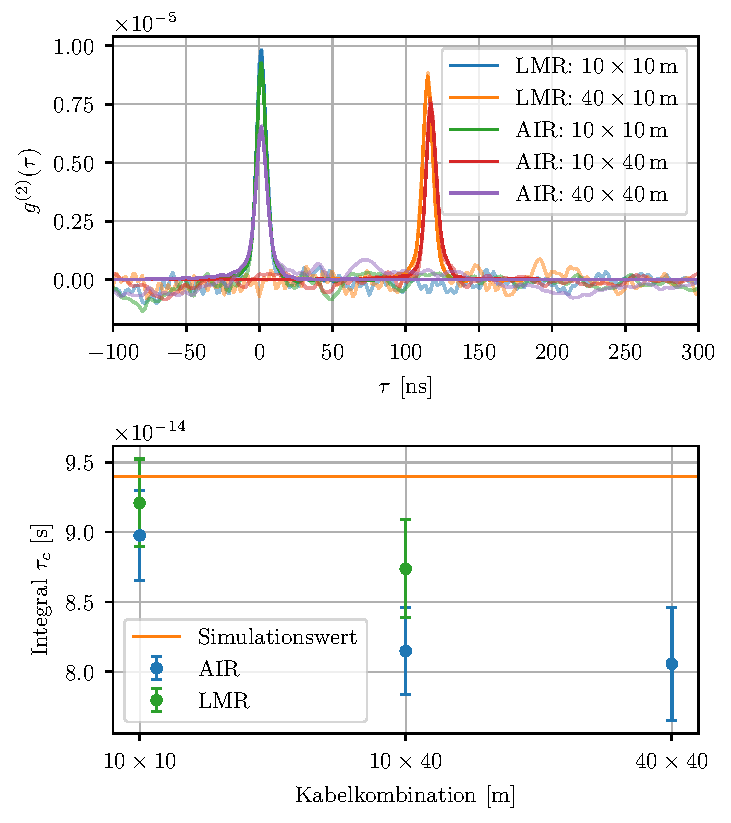
\includegraphics{images/Analysis/all_combined.pdf}
    \caption{Dargestellt sind oben die gemittelten $g^{(2)}$-Funktionen und Fits und unten die resultierenden Integrale und Fehler für alle verwendeten Kabelkombinationen.}
    \label{fig:integrale ergebnisse}
\end{figure}
Im obigen Graph ist qualitativ erneut erkennbar, dass die Peaks eine geringere Amplitude aufweisen, je länger die kombinierte Kabellänge ist. 
Dies deckt sich mit bisherigen Resultaten von H.E.S.S. \cite{zmijaFirstIntensityInterferometry2023}. 
Weiterhin auffällig ist, dass der Peak für ungleiche Kabellängen von der Null verschoben ist. 
Dies stimmt mit der Erwartung überein, da das Signal eines Kanals vor der Korrelation eine um die Kabellängendifferenz erhöhte Strecke durchläuft. 
Unter Berücksichtigung der Ausbreitungsgeschwindigkeiten im Kabel von 84 bzw. 87\% der Lichtgeschwindigkeit für Airborne 5 bzw. LMR 400 \cite{s.r.lAirborne10Coaxial,LMR400CoaxCable} erklärt sich so die gemessene Verschiebung um etwa 115\,ns. 
Im unteren Teil der \autoref{fig:integrale ergebnisse} ist zu sehen, wie sich die Integrale bei gegebener Kabelkombination verhalten. 
Der berechnete Wert der Integrale nimmt mit steigender Dämpfung der verwendeten Kabel ab. 
So weisen kürzere Kabelkombinationen längere und längere Kombinationen kürzere Kohärenzzeiten auf. 
Weiterhin sind die Integrale der LMR-Kabel, welche eine geringere Dämpfung des Signals aufweisen, stets höher als die der Airborne-Kabel. 
Durch Betrachten des als horizontale Linie eingezeichneten, in \autoref{sec:Aufbau} bestimmten Erwartungswerts an die Kohärenzzeit wird dies nochmals verdeutlicht. 
Es scheint, als würde eine Kombination idealer $0\times 0\,\mathrm{m}$ langer Kabel eine Kohärenzzeit ergeben, welche sich gut mit der Simulation deckt. \\
Allerdings muss mit obiger Interpretation vorsichtig umgegangen werden. 
Es ist zu betonen, dass diese Ergebnisse lediglich ein Indiz für die erwähnte Abhängigkeit der Kohärenzzeit von der Kabeldämpfung darstellen. 
Betrachtet man die eingezeichneten Fehlerbalken, welche aufgrund der Überlegungen in \autoref{ssec:Fehler von tau_c} 1-$\sigma$-Intervallen entsprechen, ist festzustellen, dass die Unterschiede der Integrale nicht statistisch signifikant sind. 
Besonders zwischen den Datenpunkten $10\times 40\,\mathrm{m}$ und $40\times 40\,\mathrm{m}$ ist im Rahmen der Unsicherheit kein Unterschied festzustellen. 
Auch wenn sich die Fehlerbalken der erwähnten Messungen nicht mit der $10\times 10\,\mathrm{m}$-Messung decken, ist dies nicht automatisch auf einen Unterschied von $\tau_c$ zurückzuführen. 
Schließlich ist die Bedeutung der Fehlerbalken vielmehr, dass jeder aufgetragene Punkt bei einer Wiederholung der Messung in etwa 32\% der Fälle außerhalb der Fehlerbalken liegt. 
Zusammenfassend lässt sich also kein statistisch signifikanter Einfluss der Kabellänge bzw. Dämpfung der Kabel auf den Wert von $\tau_c$ feststellen. 
Allerdings bleibt zu erwähnen, dass sich die Abnahme der Integralwerte für steigende kombinierte Kabellänge in allen von der Arbeitsgruppe bisher durchgeführten Experimenten zeigt. \todo{Cite personbal correspondance?}
Auch wenn die vorgestellten Ergebnisse dies nicht einwandfrei beweisen können, gibt es daher deutliche Indize für einen bisher unbekannten Einfluss. 
Langzeitmessungen mit höherer Statistik sind vonnöten, um statistisch aussagekräftigere Ergebnisse zu erhalten. 
Mit diesen ließe sich besser verstehen, ob es einen Effekt gibt -- wenn ja, woher dieser genau kommt und an welchem Punkt der Signalverarbeitung er sich auswirkt. 
Während, wie in \autoref{ssec:Intensitätsinterferometrie} beschrieben, ein direkter Einfluss einer zeitunabhängigen Dämpfung auf $g^{(2)}$ theoretisch nicht zu erwarten ist, ist z. B. eine Dämpfungsabhängigkeit an einem einzelnen Schritt im komplizierten Pre-Processing der Daten durchaus nicht auszuschließen und bedarf weiterer Untersuchung mit statistisch aussagekräftigeren Daten. 

\begin{table}[h]
    \centering
    \begin{tabular}{|c|c|c|} \hline
        Kabeltyp    & Kabellänge [m] & Kohärenzzeit [fs]  \\\hline
        LMR 400     & $10\times 10$  & $92{,}1 \pm 3{,}1$ \\\hline
        LMR 400     & $10\times 40$  & $87{,}4 \pm 3{,}5$ \\\hline
        Airborne 5  & $10\times 10$  & $89{,}8 \pm 3{,}2$ \\\hline
        Airborne 5  & $10\times 40$  & $81{,}5 \pm 3{,}1$ \\\hline
        Airborne 5  & $40\times 40$  & $80{,}6 \pm 4{,}0$ \\\hline
    \end{tabular}
    \caption{Aufgelistet sind die bestimmten Kohärenzzeiten und Fehler für die verwendeten Kabelkombinationen. Die theoretische Erwartung liegt bei $\tau_c^{\mathrm{meas}}=94\,\mathrm{fs}$, vgl. \autoref{sec:Aufbau}}.
    \label{tab:gemessene Kohärenzzeiten}
\end{table}
Aus den Fits lassen sich weiterhin Werte für die Parameter $\sigma$ extrahieren welche, wie in \autoref{ssec:Fitfunktion} beschrieben, eine zusätzliche Verbreiterung des Bunching Peaks im Vergleich zur Kalibrationsmessung beschreiben. 
Die Ergebnisse, die sich aus den durchgeführten Fits für den Parameter $\sigma$ ergeben, liegen in etwa im Bereich von $0{,}05\,ns$ bis $0{,}8\,\mathrm{ns}$. 
Betrachtet man hierzu \autoref{fig:Fitfuktion für verschiedene sigma}, fällt auf, dass die resultierende Fitfunktion bei solch kleinen $\sigma$ praktisch den korrelierten mittleren Pulsen entspricht, die Faltung in diesem Fall also praktisch keinen Einfluss hat. 
Aus diesem Grund ist es der Fitroutine für die in \autoref{fig:integrale ergebnisse} dargestellten Fits auch nicht möglich, den Fehler auf $\sigma$ abzuschätzen, weshalb die oben genannten Werte für $\sigma$ nicht als tatsächliche Resultate zu interpretieren sind. 
Stattdessen sollte aus diesen der Schluss gezogen werden, dass es keine nennenswerten Einflüsse während der Messung gibt, die zu einer Verbreiterung des Bunching Peaks führen und zur Kalibration noch nicht vorliegen. 
Für Labormessungen lässt sich also abschließend festhalten, dass die Faltung mit einer Gaußfunktion überflüssig (aber nicht falsch) ist und der Fit der korrelierten PMT-Pulse ausreichend ist. 
Dies ist allerdings keineswegs allgemein gültig, wie im folgenden Abschnitt gezeigt wird.

\subsection{Vergleich mit Daten der H.E.S.S. Kampagne 2022}
\label{ssec:Vergleich mit Hess}
Als Abschluss der Analyse werden die erhaltenen Ergebnisse aus vorigem Abschnitt noch mit den zwischen 19. und 21.4.2022 an den H.E.S.S. Teleskopen gemessenen Daten für Shaula verglichen. 
Dieser Vergleich dient als Indiz dafür, ob sich die gemessenen Unterschiede von $\tau_c$ für verschiedene Kabellängen mit den obig präsentierten Laborergebnissen decken. 
Wäre dies der Fall, würde das darauf hinweisen, dass in beiden Fällen möglicherweise derselbe Effekt vorliegt. 
Die Daten jeder Kabellängenkombination sowie der mittleren Pulsformen werden über die erwähnten drei Nächte zuerst gemittelt und gespeichert. 
Anschließend werden die gemittelten $g^{(2)}$-Funktionen von Shaula mit der oben beschriebenen Methode gefittet und integriert, um möglichst vergleichbare Ergebnisse zu den Labormessungen zu schaffen. 
Die so ermittelten Ergebnisse sind erneut als Graph (\autoref{fig:integration shaula}) sowie tabellarisch (\autoref{tab:Kohärenzzeiten Shaula}) dargestellt. 
\begin{figure}[h]
    \centering
    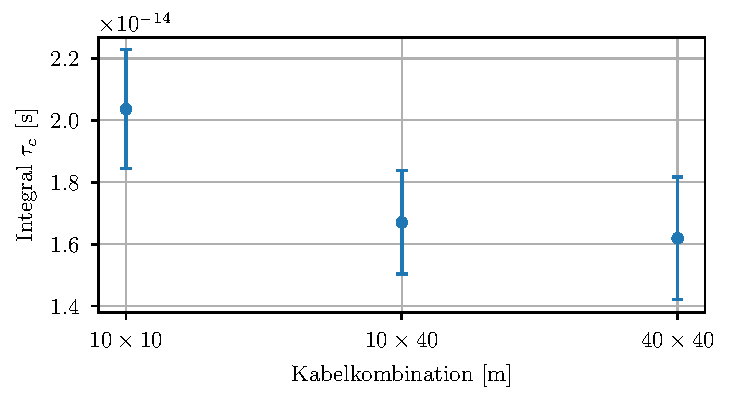
\includegraphics{images/Analysis/shaula_integrals.pdf}
    \caption{Gezeigt sind die berechneten $\tau_c$ die sich bei Integration der Shaula-Daten ergeben.}
    \label{fig:integration shaula}
\end{figure}
\begin{table}[h]
    \centering
    \begin{tabular}{|c|c|c|} \hline
        Kabeltyp    & Kabellänge [m] & Kohärenzzeit [fs]  \\\hline
        Airborne 5  & $10\times 10$  & $20{,}3 \pm 1{,}9$ \\\hline
        Airborne 5  & $10\times 40$  & $16{,}7 \pm 1{,}7$ \\\hline
        Airborne 5  & $40\times 40$  & $16{,}2 \pm 2{,}0$ \\\hline
    \end{tabular}
    \caption{Aufgelistet sind die bestimmten Kohärenzzeiten und Fehler für die verwendeten Kabelkombinationen bei der H.E.S.S.-Messung von Shaula. Für die Messung wurden Kabel des Typs Airborne 5 verwendet \cite{zmijaFirstIntensityInterferometry2023}.}
    \label{tab:Kohärenzzeiten Shaula}
\end{table}
Für einen Vergleich der beiden Messungen bietet es sich an, zu berechnen, um welchen Faktor das Integral des $10\times 40\,\mathrm{m}$-Peaks bzw. des $40\times 40\,\mathrm{m}$-Peaks kleiner ist als das Integral des $10\times 10\,\mathrm{m}$-Peaks, welches für beide Messungen am größten ist. 
Konkret wird also folgendes Verhältnis verglichen, dessen Fehler sich aus gaußscher Fehlerfortpflanzung ergibt:
\begin{equation}
    r_i = \frac{\tau_{c,10\times10}}{\tau_{c,i}} \pm \sqrt{\left(\frac{\sigma_{\tau_{c,10\times10}}}{\tau_{c,i}}\right)^2 + \left(\frac{\tau_{c,10\times10} \cdot \sigma_{\tau_{c,i}}}{\tau_{c,i}^2}\right)^2}
\end{equation}
Hierbei ist $\tau_{c,i}$ die Kohärenzzeit für die $10\times 40\,\mathrm{m}$-Messung bzw. die $40\times 40\,\mathrm{m}$-Messung und $\sigma_{\tau_{c,i}}$ der jeweilige Fehler darauf. 
Als Ergebnis für beide Raten und beide Messungen ergeben sich die in \autoref{tab:labor shalua r} gelisteten Werte. 
\begin{table}[h]
    \centering
    \begin{tabular}{|c|c|c|}\hline
        Kabellänge $i$ [m]       & Ergebnis Labor      & Ergebnis Shaula     \\\hline
        $10\times 40$            & $1{,}10 \pm 0{,}06$ & $1{,}22 \pm 0{,}17$ \\\hline
        $40\times 40$            & $1{,}11 \pm 0{,}07$ & $1{,}26 \pm 0{,}19$ \\\hline
    \end{tabular}
    \caption{Vergleichend dargestellt sind die Ergebnisse für die Raten $r_i$ bei den Labormessungen und Shaula.}
    \label{tab:labor shalua r}
\end{table}
Die Werte für das Labor $L$ und für Shaula $S$ sind innerhalb ihrer Unsicherheit verträglich, wenn die Differenz $S-L$ innerhalb ihres Fehlers $\sqrt{\sigma_L^2 + \sigma_L^2}$ auf Null abfällt. 
Da dies für beide Kabellängenkombinationen gegeben ist, lässt sich folgern, dass die Unterschiede in $\tau_c$ -- sollten sie denn existieren, was aufgrund der großen Fehler nicht als gesichert angenommen werden kann -- für Labormessungen und Messungen an den H.E.S.S.-Teleskopen im  gleichen Rahmen auftreten. 
Es gibt also ein deutliches Indiz dafür, dass bei beiden Aufbauten die Änderung im Integral (sollte sie existieren) durch das gleiche, vom Teleskop unabhängige Phänomen hervorgerufen wird. \\

Aus den Fits an die Shaula-Daten lassen sich zudem die Fitparameter $\sigma$, sowie deren Fehler extrahieren. 
Aufgrund der niedrigeren Zeitauflösung der Teleskope im Vergleich zum Laboraufbau wird erwartet, dass dieser im Bereich einstelliger Nanosekunden liegt. 
Dies liegt daran, dass Photonen, die auf die Spiegel der H.E.S.S.-Teleskope treffen, unterschiedlich lange Wege zurücklegen müssen, bis sie an den PMTs detektiert werden können. 
Daraus folgt eine Verschlechterung der Zeitauflösung im Vergleich zur Kalibrationsmessung, welche, wie in \autoref{ssec:Fitfunktion} angesprochen, zu einem Verwaschen des Bunching Peaks führt, das durch den Parameter $\sigma$ im Fit erfasst wird. 
Aus den Fits ergeben sich die in \autoref{tab:sigma Shaula} dargestellten Werte, aus denen unter Verwendung eines mit dem Einzelfehler der Werte gewichteten Mittelwerts folgt: 
\begin{equation}
    \overline{\sigma} = 2{,}01 \pm 0{,}20\,\mathrm{ns}
\end{equation}
\begin{table}[h]
    \centering
    \begin{tabular}{|c|c|}\hline
        Kabellänge $i$ [m] & Zeitauflösung [ns]  \\\hline
        $10\times 10$      & $2{,}51 \pm 0{,}32$ \\\hline
        $10\times 40$      & $1{,}15 \pm 0{,}44$ \\\hline
        $40\times 10$      & $1{,}71 \pm 0{,}45$ \\\hline
        $40\times 40$      & $2{,}23 \pm 0{,}47$ \\\hline
    \end{tabular}
    \caption{Dargestellt sind die aus den Fitparametern $\sigma$ und deren Fehlern extrahierten Zeitauflösungen für verchiedene Kabellängen.}
    \label{tab:sigma Shaula}
\end{table}
Der ermittelte Wert ist ähnlich groß wie die Zeitauflösung der H.E.S.S.-Teleskope aufgrund der verschieden langen Lichtwege, welche etwa bei $1,4\,\mathrm{ns}$ (RMS) liegt \cite{bernlohrOpticalSystemImaging2003}. 
\todo{wie hängen rms und sigma zusammen?}
\clearpage
\mbox{}
\clearpage

\section{Zusammenfassung und Fazit}
\label{sec:Fazit}
In diesem Abschnitt sollen die wichtigsten Erkenntnisse dieser Arbeit noch einmal zusammengefasst werden und ausgehend davon ein Ausblick für weitere mögliche Messungen gegeben werden. \\

Die Datenauswertung begann nach dem Pre-Processing der Einzeldateien mit der Subtraktion des niederfrequenten Störsignals. 
Hier wurde ein Tiefpass angewandt, um das Muster der Xenonlampe zu extrahieren und es abschließend vom Signal abzuziehen. 
Obwohl die Methode, wie sie hier durchgeführt wurde, zu nicht vernachlässigbaren systematischen Fehlern im niedrigen einstelligen Prozentbereich führt, ergibt sich durch diese eine effiziente Erfassung des Störsignals, was die spätere Integration und besonders die Fehlerbestimmung erst ermöglicht. 
Weiterhin vorteilhaft ist die Bestimmung des Störsignals im Frequenzraum, wodurch dieses weniger stark von hochfrequenten Signalen großer Amplitude beeinflusst wird als beispielsweise ein Fit. 
Ein Tiefpass stellt daher einen guten Weg dar, das im Labor auftretende Störsignal der Lampe zu entfernen. 
Allerdings sollte, falls es zu weiteren Labormessungen unter der Anwendung dieser Methode kommen sollte, die Wahl der Grenzfrequenz des Tiefpasses systematisch untersucht werden. 
Wie erwähnt, wurde die in der obigen Analyse beschriebene Grenzfrequenz vereinfachend visuell gewählt, wodurch sich nicht genau sagen lässt, ob diese optimal bzgl. der in \autoref{ssec:Beseitigung des niederfrequenten Störsignals} definierten Kriterien ist.
Weiterhin lässt sich nicht genau quantifizieren, wie groß der entstehende systematische Fehler tatsächlich ist, sodass lediglich eine grobe Abschätzung getroffen werden konnte. \\
Nach der Offset-Korrektur erfolgte die Wahl der Fitfunktion als Faltung der korrelierten PMT-Pulse mit einer Gaußfunktion. 
Diese Methode funktioniert für die im Labor aufgenommenen Daten mit hohem Signal-Rausch-Verhältnis und auch für die Shaula-Daten von 2022 mit geringerem Signal-Rausch-Verhältnis sehr gut. 
Fits konvergieren für beide Fälle sowohl für $\tau_\mathrm{c}$ als auch für die Fehlerbestimmung problemlos, was darauf hinweist, dass die Anwendung dieser (im Vergleich zum Gaußfit komplizierteren) Methode einfach umsetzbar ist. 
Zudem weist diese Methode einige Vorteile auf. 
Sie erfasst eine asymmetrische, PMT- und kabelabhängige Form des Bunching Peaks, wodurch diese auch in der Integration berücksichtigt wird. 
Weiterhin lässt sich über den Fitparameter $\sigma$ ermitteln, ob es zusätzliche Veränderungen der Zeitauflösung während der Messung gibt. 
Auch wenn dies nicht der Fall ist, ist die Konvergenz der Fits gut, lediglich die Fehler auf einzelne Fitparameter sind durch die Fitroutine nicht mehr abschätzbar (vgl. \autoref{ssec:Ergebnisse für verschiedene Kabelkombinationen}). 
Die gefaltene Fitfunktion weist darüber hinaus genauso viele freie Parameter wie eine Gaußfunktion auf, von denen Amplitude und Mittelwert zudem analog interpretiert werden können. 
Daher ist zu erwarten, dass die hier präsentierte Funktion auch für Daten mit niedriger Statistik ähnlich gut konvergiert wie eine Gaußfunktion, dabei aber oben genannte Vorteile aufweist und zudem am ehesten der theoretischen Erwartung an die Form des Peaks entspricht. 
Eine weitergehende Auseinandersetzung mit der Funktion in weiteren Labormessungen oder Daten von H.E.S.S. wäre daher interessant. 
Auch ein Festlegen des Parameters $\sigma$, wie er für die Auswertung der Daten in \cite{zmijaFirstIntensityInterferometry2023} erfolgt ist, wäre grundsätzlich denkbar und bedarf weiterer Untersuchung. \\
In einem kurzen Exkurs wurde daraufhin aufgezeigt, dass ein Fit für den Vergleich von Absolutwerten von $\tau_\mathrm{c}$, besonders auch für verschiedene Kabelsorten, notwendig ist. 
Die Integration von Rohdaten führt, auch bei vergleichsweise gerigem Rauschen, zu großen Abweichungen im Wert für die Kohärenzzeit, abhängig von der Integrationsbreite. 
Dies liegt zu großen Teilen an der Korrelation benachbarter Bins, wodurch breite, niedrige oder hohe Fluktuationen im Funktionswert von $g^{(2)}$ entstehen. 
Sollte eine direkte Datenintegration weiterverfolgt werden, sind daher eine Quantifizierung dieses Rauschens und eine Beschäftigung mit der Wahl der Integrationsbreite unabdingbar. \\
Daraufhin erfolgte die Abschätzung des Fehlers durch Verschiebung des Bunching Peaks über die $g^{(2)}$-Baseline, erneuten Fit und Integration. 
Es wurde gezeigt, dass durch dieses Vorgehen sinnvoll der Fehler auf $\tau_\mathrm{c}$ bestimmt werden kann, was durch eine simple Fortpflanzung der Fehler auf jeden $g^{(2)}$-Wert auf den Fit aufgrund der Korrelation benachbarter Punkte nicht möglich wäre. 
Stattdessen wurde durch die verwendete Methode das Rauschen der Baseline direkt mit in die Fehlerberechnung einbezogen, indem die Änderung des Integrals, abhängig von seiner zufälligen Position im Rauschen, berücksichtigt wurde. \\
Danach wurde die entwickelte Datenanlyse auf gemessene Daten für fünf verschiedene Kabelkombinationen der Kabel Airborne 5 und LMR 400 angewandt. 
Die Ergebnisse der Kohärenzzeiten weisen, wie bisherige Messungen der Arbeitsgruppe, weiter auf einen Einfluss der Kabellänge (z. B. durch die verschiedene Dämpfung in den Kabeln) auf den Wert von $\tau_\mathrm{c}$ hin. 
Allerdings kann dieser Einfluss keinesfalls als gesichert angenommen werden, da die Fehler trotz etwa 9{,}5-stündiger Messung immer noch zu groß sind. 
Soll dem Einfluss der Kabellänge weiter nachgegangen werden, sind daher weitere Labormessungen nicht zu vermeiden. 
Diese deutlich längeren Messungen würden (unter der bisherigen Annahme rein statistischen Rauschens auf der Baseline) zu kleineren Fehlern auf $\tau_\mathrm{c}$ führen, wodurch sich gesichertere Aussagen über den genannten Einfluss treffen lassen würden. 
In diesem Zuge wäre auch eine erneute Begutachtung der Datenverarbeitung in \autoref{sec:Datenaufnahme und Pre-Processing}, die bisher so oder so ähnlich für alle Messungen durchgeführt wurde, relevant. 
Sollte es einen Einfluss der Kabeldämpfung auf das Signal geben, würde man von diesem, wie in \autoref{ssec:Intensitätsinterferometrie} gezeigt, eigentlich keinen Einfluss auf die $g^{(2)}$-Funktion erwarten. 
Daher sollte auch die Möglichkeit nicht ausgeschlossen werden, dass z. B. Schritte im Pre-Processing der Daten einen bisher unbekannten, dämpfungsabhängigen Einfluss auf die berechneten Integrale haben. \\
Der abschließende Vergleich mit den Daten von Shaula zeigt mehrere Dinge. 
Einerseits wird wie erwähnt deutlich, dass der verwendete Fit und die Integration auch mit Daten der H.E.S.S.-Teleskope, welche ein hohes Signal-Rausch-Verhältnis aufweisen, funktionieren. 
Weiterhin wird durch den Vergleich der Kohärenzzeitverhältnisse zwischen den beiden Messaufbauten deutlich, dass ein Einfluss (sollte er existieren) zwischen den Aufbauten verträglich ist. 
Der Vergleich stellt so ein deutliches Indiz dafür dar, dass dieser Einfluss in beiden Fällen durch denselben Effekt, beispielsweise unterschiedlich lange Kabel, bedingt ist. \\

Zusammenfassend bietet die vorliegende Arbeit, auch wenn sie dem Ziel der Bestimmung und Quantifizierung des Effekts der Kabellänge auf $\tau_\mathrm{c}$ nicht statistisch aussagekräftig gerecht werden kann, weitere deutliche Indize für diesen und entwickelt auf dem Weg dahin weitere Analyseschritte, welche für weitere Messungen zur Verfügung stehen. 



\clearpage
\mbox{}
\clearpage

%---------------------------------------------------------
%	Acronyms
%---------------------------------------------------------

% \clearpage
% \mbox{}
% \clearpage
% \printnoidxglossary[type=acronym]
% \printacronyms
% \clearpage

%---------------------------------------------------------
%	Appendix (if needed)
%---------------------------------------------------------
% \clearpage
% \mbox{}
% \clearpage
% \appendix
% \addtocontents{toc}{\protect\setcounter{tocdepth}{1}}
% \addtocontents{toc}{\protect\renewcommand{\protect\sectionautorefname}{Appendix}}
% \newgeometry{
% 	%a4paper,
% 	left=40mm,
%     % right=20mm,
% 	top=15mm,
% }
%     
\section{Appendix A}
Your appendix goes here!



%---------------------------------------------------------
%	Bibliography
%---------------------------------------------------------

\newgeometry{
	%a4paper,
	left=40mm,
    % right=20mm,
	top=35mm,
}
\renewcommand\refname{Bibliography}
% \printbibliography
\printbibliography[
heading=bibintoc,
title={Bibliografie}
]

%---------------------------------------------------------
%	Danksagung
%---------------------------------------------------------

% \clearpage
% \mbox{}
% \clearpage

% \section*{Danksagung}
Here you can thank everyone you want to. 
% 
\begin{itemize}
    \item Max Mustermann for having a name that is simple to remember.
    \item Dr. Albert Einstein for having fun ideas about space-time.
\end{itemize}

%---------------------------------------------------------
%	Eigenständigkeitserklärung / Declaration of independence
%---------------------------------------------------------

% \selectlanguage{german}
\clearpage
\section*{Eigenständigkeitserklärung}
Hiermit versichere ich, Stephen Weybrecht (22967286), die vorgelegte Arbeit selbstständig und ohne unzulässige Hilfe Dritter sowie ohne die Hinzuziehung nicht offengelegter und insbesondere nicht zugelassener Hilfsmittel angefertigt zu haben. Die Arbeit hat in gleicher oder ähnlicher Form noch keiner anderen Prüfungsbehörde vorgelegen und wurde auch von keiner anderen Prüfungsbehörde bereits als Teil einer Prüfung angenommen.\\

Die Stellen der Arbeit, die anderen Quellen im Wortlaut oder dem Sinn nach entnommen wurden, sind durch Angaben der Herkunft kenntlich gemacht. Dies gilt auch für Zeichnungen, Skizzen, bildliche Darstellungen sowie für Quellen aus dem Internet.\\

Mir ist insbesondere bewusst, dass die Nutzung künstlicher Intelligenz verboten ist, sofern diese nicht ausdrücklich als Hilfsmittel von dem Prüfungsleiter bzw. der Prüfungsleiterin zugelassen wurde. Dies gilt insbesondere für Chatbots (insbesondere ChatGPT) bzw. allgemein solche Programme, die anstelle meiner Person die Aufgabenstellung der Prüfung bzw. Teile derselben bearbeiten könnten.\\

\vspace{10cm}
\begin{flushleft}
\makebox[.4\textwidth]{\hrulefill}\hfill \makebox[.4\textwidth]{\hrulefill}\\
\makebox[.4\textwidth]{Ort, Datum}\hfill
\makebox[.4\textwidth]{Unterschrift}\\
\end{flushleft}


\end{document}

